\documentclass[12pt]{article}\usepackage[]{graphicx}\usepackage[dvipsnames]{xcolor}
% maxwidth is the original width if it is less than linewidth
% otherwise use linewidth (to make sure the graphics do not exceed the margin)
\makeatletter
\def\maxwidth{ %
  \ifdim\Gin@nat@width>\linewidth
    \linewidth
  \else
    \Gin@nat@width
  \fi
}
\makeatother

\definecolor{fgcolor}{rgb}{0.345, 0.345, 0.345}
\newcommand{\hlnum}[1]{\textcolor[rgb]{0.686,0.059,0.569}{#1}}%
\newcommand{\hlstr}[1]{\textcolor[rgb]{0.192,0.494,0.8}{#1}}%
\newcommand{\hlcom}[1]{\textcolor[rgb]{0.678,0.584,0.686}{\textit{#1}}}%
\newcommand{\hlopt}[1]{\textcolor[rgb]{0,0,0}{#1}}%
\newcommand{\hlstd}[1]{\textcolor[rgb]{0.345,0.345,0.345}{#1}}%
\newcommand{\hlkwa}[1]{\textcolor[rgb]{0.161,0.373,0.58}{\textbf{#1}}}%
\newcommand{\hlkwb}[1]{\textcolor[rgb]{0.69,0.353,0.396}{#1}}%
\newcommand{\hlkwc}[1]{\textcolor[rgb]{0.333,0.667,0.333}{#1}}%
\newcommand{\hlkwd}[1]{\textcolor[rgb]{0.737,0.353,0.396}{\textbf{#1}}}%
\let\hlipl\hlkwb

\usepackage{framed}
\makeatletter
\newenvironment{kframe}{%
 \def\at@end@of@kframe{}%
 \ifinner\ifhmode%
  \def\at@end@of@kframe{\end{minipage}}%
  \begin{minipage}{\columnwidth}%
 \fi\fi%
 \def\FrameCommand##1{\hskip\@totalleftmargin \hskip-\fboxsep
 \colorbox{shadecolor}{##1}\hskip-\fboxsep
     % There is no \\@totalrightmargin, so:
     \hskip-\linewidth \hskip-\@totalleftmargin \hskip\columnwidth}%
 \MakeFramed {\advance\hsize-\width
   \@totalleftmargin\z@ \linewidth\hsize
   \@setminipage}}%
 {\par\unskip\endMakeFramed%
 \at@end@of@kframe}
\makeatother

\definecolor{shadecolor}{rgb}{.97, .97, .97}
\definecolor{messagecolor}{rgb}{0, 0, 0}
\definecolor{warningcolor}{rgb}{1, 0, 1}
\definecolor{errorcolor}{rgb}{1, 0, 0}
\newenvironment{knitrout}{}{} % an empty environment to be redefined in TeX

\usepackage{alltt}
\usepackage{amsmath,amsfonts,amssymb,graphicx,authblk}
\usepackage[font={footnotesize,singlespacing},labelfont=bf]{caption}
\usepackage{titlesec,blkarray, bm} 
\usepackage{float,afterpage}
\usepackage[running,mathlines]{lineno}
\usepackage[vmargin=1in,hmargin=1in]{geometry}
\usepackage[authoryear,sort]{natbib}
\usepackage[dvipsnames]{xcolor}
\usepackage[nodisplayskipstretch]{setspace} 
\usepackage{hyperref}
\usepackage[section]{placeins}
\usepackage{gensymb}
\usepackage{enumitem}
\usepackage{orcidlink}
\usepackage{tabularx} % put this once in your preamble
\usepackage{booktabs}
\usepackage{pdflscape}  % or \usepackage{lscape}
\usepackage{adjustbox}
\usepackage{newfloat}   % for creating new float types
\usepackage{tocloft}    % for customizing lists
\usepackage{caption}
%\usepackage{hyperref}
\setlist{topsep=.125em,itemsep=-0.15em,leftmargin=0.75cm}
\setlength{\parindent}{0.35in}

\usepackage[sc]{mathpazo} %Like Palatino with extensive math support
\usepackage[subtle]{savetrees}

\usepackage{lineno}
%\renewcommand{\refname}{Literature Cited}
%\renewcommand{\floatpagefraction}{0.9}
%\renewcommand{\topfraction}{0.99}
%\renewcommand{\textfraction}{0.05}

\clubpenalty = 10000
\widowpenalty = 10000

\sloppy 

\usepackage{ifpdf}
\ifpdf
\DeclareGraphicsExtensions{.pdf,.png,.jpg}
\DeclareFloatingEnvironment[fileext=losf, listname={List of Supplementary Figures}]{suppfigure}
\DeclareFloatingEnvironment[fileext=lost, listname={List of Supplementary Tables}]{supptable}
\usepackage{epstopdf}
\else
\DeclareGraphicsExtensions{.eps}
\fi

%\graphicspath{{/Users/jacobmoutouama/Dropbox/Miller Lab/github/endo-range-limits/Figure}}
%\graphicspath{{C:/Users/tm9/Dropbox/github/ELVI-endophyte-density/Figure}}
\newcommand{\tom}[2]{{\color{red}{#1}}\footnote{\textit{\color{red}{#2}}}}
\newcommand{\jacob}[2]{{\color{blue}{#1}}\footnote{\textit{\color{blue}{#2}}}}
\renewcommand\Authfont{\normalfont\normalsize}    % sets author names to small
\renewcommand\Affilfont{\normalfont\small} % sets affiliations even smaller
\renewcommand{\thesuppfigure}{S\arabic{suppfigure}}
\renewcommand{\thesupptable}{S\arabic{supptable}}
\setlength{\affilsep}{1em}  
%\doublespacinq



% I cannot get \orcidlink working on my computer so for now replacing this with \textit

%-------------------------------------------------------------------------
\title{\Large When mutualism weakens: stress alters endophyte benefits in cool-season grasses}
\author[1]{Jacob K. Moutouama\,\orcidlink{0000-0003-1599-1671} \thanks{Corresponding author: jmoutouama@gmail.com}}
\author[2]{Josh C. Fowler}
\author[3]{Akiem Gough}
\author[3]{Julia Martin}
\author[3]{Chris Oxley}
\author[3]{Karl Schrader}
\author[3]{Karis Williams}
\author[3]{Tom E.X. Miller\,\orcidlink{0000-0003-3208-6067}}

\affil[1]{Department of Botany, University of British Columbia, Vancouver, BC, Canada}
\affil[2]{Department of Environmental Studies, University of Colorado Boulder,Boulder,CO, USA}
\affil[3]{Program in Ecology and Evolutionary Biology, Department of BioSciences, Rice University, Houston, TX,USA}
\date{} % clear date


\sloppy

%-------------------------------------------------------------------------
\IfFileExists{upquote.sty}{\usepackage{upquote}}{}
\frenchspacing
\begin{document}
%\SweaveOpts{concordance=TRUE}
\renewcommand{\baselinestretch}{1.2}
\maketitle
% \bigskip 
%45 character limit on running head
\noindent\textbf{Running header:} Stress and Grass–Endophyte Interactions
\bigskip 

\noindent\textbf{Keywords:} demography, mutualism, parasitism, plant–fungi interactions, range limits, stress gradient hypothesis

\bigskip 
\noindent\textbf{Submitted to:} \textit{Ecology letters} (Letter)

\bigskip 
\noindent\textbf{Data accessibility statement:} 
If the paper is accepted, all data and computer scripts supporting the results will be archived in a Zenodo package, with the DOI included at the end of the article. 
During peer review, all data files required to reproduce the analyses, including annual census data, are temporarily hosted via Dropbox and available at 
\url{https://www.dropbox.com/scl/fo/fgxng2mcemjyv41bihul9/AGiZs5mPRGcCZURpGyvhjCE?rlkey=7mgdyrus3ga44yj3ygfncfmkd&dl=1}. 
All analysis scripts (Stan and R) are available at \url{https://github.com/jmoutouama/endo-range-limits}.

\bigskip 
\noindent\textbf{Conflict of interest statement:} None.

\bigskip
\noindent\textbf{Acknowledgments}
This research was supported by National Science Foundation Division of Environmental Biology award 2208857.


\bigskip
\noindent\textbf{Authorship statement:}
%J.K.M., A.C. and T.E.X.M. designed the study.
%A.C. and T.E.X.M. collected the data. 
%All authors conducted the statistical analyses and modeling.
%J.K.M. drafted the manuscript, and T.E.X.M contributed to revisions.

\bigskip
\noindent\textbf{Abstract:}\\
\noindent\textbf{Main Text:}\\
\noindent\textbf{Figures: 5}\\
\noindent\textbf{Tables: 1}\\
\noindent\textbf{References: X}

\newpage
%\SweaveOpts{concordance=TRUE}
\linenumbers
%-------------------------------------------------------------------------
\spacing{1.25}
\section*{Abstract}
%150 words limit for Ecology letter. The number now is 146
%Beneficial plant-fungal interactions are widespread and crucial for terrestrial ecosystems. 
Benefits of plant-microbe symbioses are predicted to increase under environmental stress, but the relative roles of abiotic and biotic factors as modifiers of symbiotic interaction outcomes remain unclear.
We studied how the independent and combined effects of aridity and herbivory modify the demographic effects of seed-transmitted fungal endophytes on three native grass host species using geographically distributed field experiments along a precipitation gradient, crossed with herbivore exclusion. 
Host demographic performance declined under lower precipitation, with endophyte-symbiotic plants having nearly twice the mortality risk of non-symbiotic plants, \tom{and spikelet production was frequently reduced under such stressful conditions}{Unclear whether this is a statement about symbiont effects, or abiotic effects, or both.}.
\tom{Herbivory had only occasional effects on plant–microbe symbioses.}{Can you add a little more detail to this statement? It's pretty vague.} 
In contrast, abiotic stress emerged as the primary driver of symbiosis outcomes, but in the opposite direction than predicted by theory and previous studies, with symbioses becoming more beneficial in more benign abiotic environments.
These results highlight that symbiotic fungi can become liabilities under stress, with implications for the dynamics of plant-fungal mutualisms under global change.

%--------------------------------------------------------------------
\newpage
\section*{Introduction}
Symbiotic mutualisms are widespread and ecologically important, occurring across plant and animal hosts, and often mediating key ecological functions such as stress tolerance and defense against natural enemies. 
These interactions are famously context-dependent, with the direction and strength of outcomes shaped by the environment in which they occur \citep{hoeksema2015context, bronstein1994conditional,hoang2024impacts}. 
The stress-gradient hypothesis (SGH) is a classic and influential framework for predicting the context-dependency of interaction outcomes, predicting that positive interactions increase under stressful conditions \citep{louthan2015and,bertness1994positive,holmgren2010strong}.
%, but actual outcomes depend on the type and intensity of biotic and abiotic stress
For example, microbial symbionts that benefit host plants under drought stress may become neutral or even parasitic under more benign conditions \citep{giauque2019endophyte}. 
%Variation in the nature and intensity of biotic and abiotic stress is thus a key driver of these context-dependent outcomes. 

\tom{Because microbial symbioses}{This is a plant paragraph -- without really signaling it, you have narrowed the scope of the paper to just plants and microbes. This is fine, but I think it means you should open the intro with a focus on plants and microbes. Alternatively, you can keep this paragraph more general by talking about ``natural enemies'' (rather than ``herbivory''), and using more examples from the animal literature. Obviously, at some point the Intro will need to narrow down to plants and endophytes, but you will keep a broad audience if you can frame the study more broadly.} are expected to become more beneficial in stressful conditions, they can substantially enhance host resilience to environmental stress.
Under biotic stress, such as herbivory, microbial symbiosis can benefit host plants by facilitating the production of secondary compounds that deter feeding or exert direct toxicity, thereby reducing herbivore growth, survival, and oviposition \tom{\citep{atala2022fungal,bastias2017epichloe,vega2008insect}.}{Not only plant-microbe, but actually all the references here and in the next sentence are grass-endophyte. Again, I think there is risk in making the Intro too narrow too early. } 
Similarly, under abiotic stress, such as low precipitation, nutrient limitation, or high temperature, symbiotic microbes can enhance host tolerance through a variety of mechanisms \citep{clay2002evolutionary, afkhami2008symbiosis}. 
Microbial symbionts of plants, including mycorrhizae, rhizobia, and endophytic bacteria and fungi, can improve water and nutrient acquisition by increasing root surface area, facilitating nutrient mobilization, or promoting nitrogen fixation, allowing plants to maintain growth and metabolic function under drought or poor soil conditions \citep{amijee1989development}.
In addition, many symbiotic microbes stimulate the production of antioxidant enzymes, which reduce oxidative damage caused by stressors like drought, salinity, and heat \citep{ruiz1996superoxide}. 
\tom{By improving resource acquisition, modulating plant physiology, and enhancing stress-responsive metabolism, these symbiotic interactions help host plants buffer against environmental stochasticity and extreme conditions across a wide range of ecosystems \citep{fowler2023geographic}.}{There are recent review papers on microbial mediation of climate stress by Jenn Rudgers, Michelle Afkhami, and collaborators that are relevant to cite here or elsewhere. I will try to find those and send them to you.}

%Although microbial symbioses often enhance plant performance, they can also impose substantial costs, particularly in resource-limited environments. 
While stress is hypothesized to strengthen the benefits of symbiotic microbes, growing evidence suggests that it could also elevate costs of symbiosis.
Maintaining symbionts requires that hosts allocate valuable carbon and nutrients to sustain their microbial partners.
For instance, mycorrhizal fungi may require up to 20\% of a host's photosynthetically fixed carbon \citep{thirkell2020carbon,soudzilovskaia2015quantitative}, and under abiotic stress, this investment can outweigh the benefits of the symbiosis \citep{johnson1997functioning, bronstein2001exploitation}, reducing host survival, growth, reproduction, or competitive ability \citep{klironomos2003variation}. 
Similarly, vertically transmitted endophytes can shift from mutualistic to antagonistic interactions when they produce stromata that abort host inflorescences or impose energetic costs \citep{saikkonen2004evolution}. 
For example, under low nutrient or water conditions, endophyte-infected grasses may produce fewer tillers and lower total biomass compared to endophyte-free plants, reflecting the costs of sharing limited resources \citep{ahlholm2002vertically}. 
\tom{}{I think we need a sentence to close this paragraph that makes some broader point, that generates suspense, and that transitions to the next paragraph. Something about how we still don't know whether stress is more likely to elicit net benefits or net costs.}

%\tom{However, in many plant-microbe interactions, host protection is not guaranteed solely by the presence of a symbionts; rather, the density of the symbiont can determine the effectiveness of this protection \citep{laughton2014combined}. 
%Higher endophyte densities may lead to increased resource exploitation by the symbiont, potentially imposing costs on the host, such as reduced growth or reproduction \citep{faeth2009asexual}.}{I like these sentences and the idea is really interesting and important -- but if we are not using the endo density data in this paper then I would remove.}
%This cost is often manifested by a reduction in host biomass or reproductive success \citep{faeth2009asexual}, particularly under harsh abiotic conditions \citep{cui2024review}. 
%Ultimately, these context-dependent costs and benefits may underlie the observed distribution of host species.

%Mutualist limitation reduces population fitness and therefore limits range expansion in \emph{Medicago polymorpha} populations \citep{lopez2021microbial}. 
%Although context dependence, along with spatiotemporal variations in abiotic environmental conditions may reduce the effectiveness of the benefits provided by the symbiont to the host species, our understanding of the mechanisms that alter host-symbiont interactions across species geographic range remains limited.

%\tom{Despite growing interest in the ecological and evolutionary roles of symbiosis, most studies focus on the host plant’s perspective and rarely manipulate symbiont prevalence to evaluate how environmental variation shapes the symbiont’s effects on host demography across geographic ranges. 
%Yet, symbionts promote their own fitness by influencing host life history traits and enhancing resistance to stress \citep{kazenel2015mutualistic, giauque2019endophyte, saikkonen1998fungal}. 
%Theory predicts that exclusive vertical transmission fosters mutualism and leads to high symbiont prevalence in host populations \citep{fine1975vectors}. 
%Field studies suggest that, under stressful conditions, beneficial symbionts may increase in prevalence and even reach fixation if their fitness advantages outweigh reproductive costs \citep{donald2021context}. 
%However, populations with lower prevalence may experience higher symbiont loss among offspring \citep{afkhami2008symbiosis}. 
%Thus, overlooking symbiont dynamics could result in inaccurate predictions of host population responses to global change.}{Again, I really like this paragraph, but we need to think about whether and how the symbiont density data will be used here. Is that what you are pointing towards here? Otherwise I am not sure why you are bringing up symbiont prevalence, since I did not think the prevalence data were going into this paper.}

Despite growing interest in the role of symbiosis in shaping host demography, few studies have tested how abiotic and biotic stressors synergistically influence the demographic effects of symbionts. 
Furthermore, it remains unclear which of these stressors is more critical in eliciting the benefits and/or exacerbating costs of symbionts. 
Most work has been conducted in controlled or \tom{common garden experiments}{Technically we have a common garden experiment.}.
\tom{In \emph{Ammophila breviligulata}, herbivory but not drought reduced growth, and no interaction was observed; however, plants hosting endophytic fungi were more resistant to these stressors \citep{emery2010variation}.}{This sentence is hard to follow. Can you sharpen it to bring the symbiosis effect into focus?}
Studying the combined effects of abiotic and biotic stressors under natural conditions is particularly important in the context of global change \citep{louthan2015and}, as shifting climate patterns and altered herbivore pressures may change the balance of costs and benefits in plant–microbe interactions, potentially influencing species distributions and ecosystem function \citep{reynolds2003grassroots}.
Understanding how abiotic stress, biotic stress, and microbial symbiosis interact to influence plant performance requires experiments that jointly vary all three factors. 
\tom{However, to our knowledge, no such comprehensive study has been conducted.}{This is good to include, as long as we are confident that it's true. What about the Ammophila example above?}
Here, we address this gap by examining the  effects of biotic and abiotic stress on the demographic effects of endophyte symbiosis on three grass host species spanning a natural range-core/range-edge precipitation gradient.
%providing insight into how these biotic and abiotic stressors influence endophyte prevalence, host fitness component such as survival, growth and reproduction under realistic environmental conditions.

%Moreover, it remains unclear which stressor is most critical in eliciting the benefits of \tom{endophyte symbiosis}{What is the intended scope at this point in the paper? Is this meant to be a general statement about microbial symbioses, or are we now talking specifically about Epichloe symbioses in grasses? I think the Intro can provide clearer sign-posting for this. 
%There is a lot of literature on drought and herbivory in the Epichloe literature. I think it would be good to have a paragraph late in the Intro that introduces this system and briefly covers the literature on drought and herbivory, highligting that few (or no?) previous studies have looked at both.}, or how multiple stressors may interact to influence host demography. 
%Herbivory is a biotic factor that can significantly affect host fitness \citep{benning2019biotic} and mediate the outcomes of symbiotic interactions. 
%Herbivores reduce host fitness through tissue damage, defoliation, and altered resource allocation \citep{maron2006herbivory}, and can also impose indirect ecological costs by influencing reproductive or growth strategies \citep{miller2008herbivore}. 
%These ecological costs may shape the selective landscape in ways that favor symbiont persistence or transmission \citep{clay2005herbivores}. 
%For example, herbivory can enhance the fitness benefits of endophyte infection by triggering host defense pathways or promoting vertical transmission of the symbiont \citep{gundel2020simulated,agrawal1999transgenerational}. 
%If the ecological context of herbivory alters the net fitness effects of symbiosis, then interactions between herbivory and abiotic stress (e.g., drought or high temperature) may play a critical role in determining host population persistence.\tom{}{The opening sentence suggested that this paragraph would be about the combined and relative roles of abiotic and biotic stress, but most of this paragraph is actually about herbivory. Again, bring attention to the way you structure paragraphs. Use clear topic sentences, and make sure the content of the paragraph stays true to the topic sentence. }

%\tom{}{Here is where I might dedicate a paragraph to describing the biology and context-dependence of the grass-endophyte symbioses.}
%Fungal endophytes of plants provide a tractable system for studying the ecological effects and context-dependence of host-symbiont interactions, as host status (symbiotic vs symbiont-free) can be experimentally manipulated. 
%In many cases, endophyte-symbiotic grasses outperform endophyte-free grasses under water limitation, although the benefits depend on host and endophyte identity \citep{decunta2021systematic}.
%A well-studied example is the association between cool-season grasses and seed-transmitted fungal endophytes in the genus \textit{Epichloë} \citep{schardl2004symbioses,saikkonen2010defensive,oberhofer2014effects,clay2005herbivores}. 
%In the case of \textit{Epichloë}–grass interactions, vertical transmission couples host and symbiont fitness, a linkage expected to favor the evolution of mutualistic interactions \citep{gundel2024temporal,gundel2011incorporating}.
%Even with tight host–symbiont fitness coupling, the prevalence of \textit{Epichloë} infection is strongly influenced by environmental conditions, including long-term variation in precipitation and temperature \citep{rudgers2016long,fowler2025increasing}.
%Even when endophytes do not enhance survival under stress, they may still boost host fitness by promoting growth and reproduction \citep{yule2013costs}. 
%More generally, prior work has shown that effects of endophyte symbiosis may vary in magnitude and even sign across host vital rates \citep{rudgers2012there}, which argues for considering multiple life history pathways. 
%Importantly, hosting endophytes can entail costs, including the allocation of plant carbon to sustain the fungal partner and potential risks associated with horizontal transmission. 
%These costs may be offset by benefits such as herbivore deterrence, mediated by fungal alkaloids that protect against both invertebrate and vertebrate herbivores \citep{clay2005herbivores,saikkonen2010defensive}
%Together, these features make grass–\textit{Epichloë} symbioses an ideal system for investigating how abiotic stressors, such as drought, interact with biotic stressors, like herbivory, to determine the outcome of symbiosis.

Symbioses between cool-season grasses and seed-transmitted fungal endophytes (\textit{Epichloë} spp.) provide a powerful experimental model for studying how abiotic and biotic elements of ecological context influence host–symbiont interactions \citep{schardl2004symbioses,saikkonen2010defensive,oberhofer2014effects,clay2005herbivores}. 
Because vertical transmission links host and symbiont fitness, it is expected to favor the evolution of mutualistic interactions \citep{gundel2024temporal,gundel2011incorporating}. 
Environmental conditions, including long-term variation in precipitation and temperature, strongly influence both the prevalence of \textit{Epichloë} infection and the benefits conferred to hosts \citep{rudgers2016long,fowler2025increasing}. 
For example, grasses hosting endophytes often outperform endophyte-free individuals under water limitation, though the magnitude of these benefits depends on both host and symbiont identity \citep{decunta2021systematic}. 
Hosting \textit{Epichloë}  endophytes can also entail costs, such as carbon allocation to sustain the fungus or risks associated with horizontal transmission; \tom{these may be offset by benefits including herbivore deterrence via fungal alkaloids \citep{clay2005herbivores,saikkonen2010defensive}. }{I think you will want a stand-alone sentence describing fungal alkaloids and their anti-herbivore effects, including relevant citations, since this leads directly to the herbivory element of the experimental design.}
Finally, \textit{Epichloë} endophyte effects can differ across host vital rates, which makes it important to consider multiple vital rates in assessing costs and benefits: symbiosis may not improve survival under stress, but can still enhance growth and reproduction \citep{yule2013costs,rudgers2012there}. 
%Together, these features make grass-\textit{Epichloë} symbioses an ideal system for investigating how abiotic stressors, such as drought, interact with biotic stressors, like herbivory, to determine the outcome of symbiosis.
%Moreover, variation in endophyte effects across life-history pathways highlights the importance of considering multiple host traits when evaluating mutualistic outcomes \citep{rudgers2012there}.

We established experimental gardens of three species of native cool-season grasses across an aridity gradient in the south-central United States to investigate how endophyte symbiosis affects multiple host vital rates under varying abiotic and biotic stress. 
This gradient, from mesic conditions in the east to increasingly arid conditions in the west, provides a biologically realistic stress gradient, and coincides with the westernmost range limits of many eastern North American grass species. 
At each of seven sites along the gradient, we manipulated vertebrate and invertebrate herbivory (allowing herbivore access versus exclusion) to test its interaction with abiotic stress.
Across these abiotic and biotic contexts, we quantified effects of symbiosis by comparing the demographic performance of endophyte-symbiotic (E+) and endophyte-free (E-) individuals. 
We asked whether endophyte symbiosis is beneficial for host grasses, whether symbiont benefits are amplified under exposure to abiotic or biotic stressors, as predicted by the SGH, and how these two forms of stress combine to influence the demographic outcomes of endophyte symbiosis.
Specifically, we tested the following predictions (Fig.~\ref{fig:prediction}): 
\begin{enumerate}
	\item Endophyte symbiosis will generally be beneficial for the demography of these native grass hosts.
	\item Because endophytes can improve drought tolerance (e.g., by enhancing water use efficiency or root growth), they will be most beneficial in arid environments, and neutral or costly in mesic environments.
	\item Because endophytes produce defensive compounds (e.g., alkaloids), they will be most beneficial under herbivore exposure, and neutral or costly under herbivore exclusion.
	\item The combined stresses of herbivory and low precipitation will amplify the physiological demands on the host plant, such that costs of maintaining endophyte associations will dampen net benefits relative to each stressor in isolation.
\end{enumerate}
\tom{}{I updated this paragraph a bit to focus more on predictions, since that is what is shown in Figure 1 -- I changed my mind from the previous round of edits! I do like the predictions, and we should keep polishing these. I tried to include some logic for \emph{where} these predictions come from, specifically the idea of interference between abiotic and biotic stress, which is what I think is drawn in the figure (and I tried to summarize in the predictions). Has that been shown or hypothesized elsewhere? Why not predict that endophyte are most beneficial under the combined stressors, as you had in a previous draft?}
%Our analyses tested these predictions and quantified the relative importance of abiotic and biotic dimensions of environmental context as driver of variation in host-symbiont interaction outcomes. 
\tom{}{Some comments on figure one. I would more clearly label y axes, and more clearly indicate herbivore access and herbivore exclusion on the two panels. Maybe you can put a cross over the deer in the herbivore exclusion panel. Use a legend or clearer labeling to indicate which is E+ and which is E-. YOu have eight arrows on the left and right sides of the figures, and it is difficult to understand how these relate to the prediction lines. SO I think this still needs some work, but I like the general idea.}
%under reduced precipitation, do endophytes enhance host fitness by mitigating drought stress, or can they impose a net cost under extreme combined stress from drought and herbivory ? and (ii) does the relative importance of endophyte-mediated benefits change along the stress gradient, as predicted by the stress-gradient hypothesis (SGH), with higher abiotic stress amplifying mutualistic effects? 
%We predicted that endophytes would enhance host fitness under moderate drought in the absence of herbivores, representing an endophyte-driven stress amelioration scenario (Fig.~\ref{fig:prediction}A). 
%When herbivores are added as a second stress under more extreme drought, the metabolic cost of maintaining the endophyte may reduce benefits or even impose a net cost, corresponding to a reduced endophyte-mediated benefits scenario (Fig.~\ref{fig:prediction}B). 
%Overall, consistent with the SGH, endophyte-mediated benefits are expected to increase under lower precipitation, with the presence or absence of herbivores modulating these effects.

%    \item Because endophytes often produce defensive compounds (e.g., alkaloids), plants with endophytes will experience less herbivore damage and maintain higher vital rate compared to plants without endophytes  \tom{when grazed}{We do not have much direct information about `grazing'. I would keep the focus on herbivore access or exclusion, since that is what we directly measured.}.
%    \item Because endophytes can improve \tom{drought tolerance}{I would lead with the abiotic stressors, since that is more central to the experimental design.} (e.g., by enhancing water use efficiency or root growth), plants with endophytes will outperform plants without endophytes more in dry conditions than in wet conditions.
%     \item The combined stresses of herbivory and low precipitation will create conditions where the mutualistic benefits of endophytes are most pronounced, giving plants with endophytes a strong performance advantage over plants without endophytes.
%     \item The combined stresses of herbivory and low precipitation will amplify the physiological demands on the host plant, \tom{such that the additional resource costs of maintaining endophyte associations will  reduce overall plant performance resulting in endophyte-infected plants performing worse than uninfected plants under extreme stress conditions}{I am confused here because this prediction seems to contradict the preceding prediction. But either way, I still think it would be more compelling to phrase these as questions.}.
%\end{enumerate}
%--------------------------------------------------------------------
\section*{Materials and methods}
\subsection*{Study system}
Our study focused on three cool-season perennial grass species native to woodland and prairie habitats of eastern North America: \emph{Agrostis hyemalis}, \emph{Elymus virginicus}, and \emph{Poa autumnalis} (Poaceae, subfamily Pooideae) \citep{shaw2011guide}.
\emph{A. hyemalis} is a short-lived perennial that germinates from autumn to late winter and, in our Texas study region, typically flowers between April and June. 
\emph{E. virginicus} is a larger, longer-lived species that flowers throughout spring and summer. 
\emph{P. autumnalis} has a similar growth form to \emph{E. virginicus} and flowers in late spring. 
\emph{Agrostis hyemalis} hosts the endophyte \emph{Epichloë amarillans} \citep{white1994endophyte}, \emph{E. virginicus} typically hosts \emph{Epichloë elymi} \citep{liu2023fungi}, and \emph{P. autumnalis} hosts \emph{Epichloë PauTG-1} or \emph{E. typhina subsp. poae} \citep{gundel2020simulated}.
Like other \emph{Epichloë} species, these endophytes are primarily transmitted vertically through seeds and are additionally capable of horizontal transmission via sexual stromata on inflorescences or asexual conidia on leaf surfaces \citep{clay2002evolutionary, gundel2020simulated,leuchtmann2014nomenclatural}. 
In our study, stromata were never observed on \emph{E. virginicus} or \emph{Poa autumnalis} and very rarely observed on \emph{A. hyemalis} (<5\% of individuals), suggesting low levels of horizontal transmission.
Herbivory in this system is primarily from deer, generalist insects, and small mammalian grazers, which can influence both plant performance and endophyte-mediated defenses. 

\subsection*{Source populations and symbiont removal}
\tom{}{I am planning to work on the supp data for this section but for now I want to keep moving, so just editing the text.}
Plants used in our experiment were derived from natural (source) populations of each species (Fig.~\ref{fig:site}, Table~\ref{tab:source_pop}). 
\jacob{Prevalence of fungal endophytes in these natural populations ranged from XX\% to XX\% endophyte-positive hosts (NEW SUPP TABLE). }{ I am not sure about this.}
\tom{Seeds from these source populations (from ca. 30 plants per population) were either heat-treated or left untreated, intended to produce symbiont-free ($E^-$) and symbiotic ($E^+$) plants from the same genetic lineages.
For \emph{Elymus virginicus} and \emph{Poa autumnalis}, heat-treated seeds were placed in a drying over at 60°C for approximately five days. 
For \emph{Agrostis hyemalis}, seeds were heat-treated in a water bath at 60°C for 12 minutes. }{We should talk about this. You need more detail here -- I have tried adding some but there is more to do. They were all treated but not all treatments were successful, which we need to report. And there were a few different methods used on different species. This should all go in the supplement. It is also not true that heat treatment has no effect on seed viability, which is why we tried to use seeds that were multiple generations removed from the heat treatment.}
Where possible, endophyte-removal lineages were reared through at least one generation before use in experiments, to minimize the direct effects of heat treatment (Supp Table). 
All seeds, both heat-treated and non-heat-treated, were surface-sterilized with 10\% bleach solution then germinated on agar plates.
Seedlings were transferred to potting soil and grown in the Rice University greenhouse. 
Once these plants were sufficiently large in size they were scored for their endophyte status and vegetatively propagated, with clonal identities tracked across individuals. 
In total, we used 3 source populations and XX unique genotypes for \textit{A. hyemalis}, XX source populations and XX genotypes for \textit{E. virginicus}, and XX source populations and XX genotypes \textit{P. autumnalis}.
After vegetative propagation, the experiment included 840, 840, and 720 clones in total across all populations. 

Before transfer to the field experiment, we confirmed endophyte status (E$^+$ or E$^-$) of all seedlings using either microscopy or an immunoblot assay; realized numbers of E$^+$ and E$^-$ individuals per species and population are provided in Supplementary Table~\ref{tab:endo_counts}. 
We assessed endophyte status using three methods. 
First, for microscopy, peels of the inner leaf sheaths were stained with aniline blue lactic acid and viewed under a compound microscope at 200x–400x to identify \emph{Epichloë} hyphae \citep{jackson1988rapid}. 
Second, we used microscopy to assess the presence or absence of \emph{Epichloë} in seeds that were squashed and stained similarly as the leaf tissue, to determine the endophyte status of the maternal plant \citep{fowler2025increasing}. 
Third, we used an immunoblot assay (Phytoscreen field tiller endophyte detection kit, Agrinostics Ltd. Co.) that target proteins of \emph{Epichloë} spp. to visually indicate presence or absence \citep{koh2006rapid}. 
All of these approaches have proven reliable in previous studies and, in cases where two or more methods were used on the same plants in this study ($N=253$), there was 99.2\% agreement.
For genotypes that were vegetatively propagated, we tested the endophyte status of a single clonal replicate and assume that its status applies equally to all clones of a given source genotype. 

\subsection*{Common garden experimental design and climate data}
To examine the effects of endophyte symbiosis across an abiotic stress gradient, we established common garden experiments with E+ and E- hosts at seven sites along an aridity gradient from Louisiana to central Texas, US (Fig.~\ref{fig:site}, Table~\ref{tab:exp_sites}).
From west to east, mean annual precipitation increases more than three-fold across these sites while mean annual temperature is relatively consistent, \tom{based on 30-year climate normals}{True?} (Fig. \ref{Sup:temp}).
For this reason, we focus on precipitation as the primary abiotic factor that varied across sites.  
This geographic gradient overlaps and exceeds the natural range edges of our focal species, ensuring exposure to realistic climatic and biotic conditions (Fig.~\ref{fig:site}A,B, C). 

To characterize climate at these sites during the study period (2023–2025), we collected monthly temperature and precipitation data from PRISM at 800 m resolution \citep{PRISM2024}. 
For each site, we calculated mean temperature (\textdegree C) and cumulative precipitation (mm) over the corresponding census year, defined as the period from transplanting to the demographic census.
\tom{During our study period, realized precipitation at these sites corresponded well to 30-year normals, with wetter eastern sites and drier western sites (Fig.~\ref{fig:site}D).}{I suggest breaking up these bars to show years separately. The analyses use site-year climate values, so this is relevant to show.} 

At each of seven sites along the gradient, we established 24 square plots (1.5 m $\times$ 1.5 m), eight per host species (\textit{P. autumnalis} was planted at six sites, excluding the westernmost site (SON) since it is well outside this species' natural range: Fig.~\ref{fig:site}C). 
\tom{Within each site, each plot was randomly assigned to either herbivore access or herbivore exclusion (Fig.~\ref{fig:site}E). }{Can you update this cartoon to show both E+ and E- plants within the same plot?}
The herbivory treatment targeted both vertebrate and invertebrate hebivores: exclusion plots had deer fencing on four sides and were sprayed with Sevin insecticide (active ingredient Zeta-Cypermethrin) 2-3 times per growing season following the manufacturer's protocol; herbivore access plots were unsprayed and fenced on two sides to control for any fence effect.

Greenhouse-raised plants were planted into the field experiment in February-March 2023.
Each plot was planted with 15 individuals, a mix of E+ and E- host-plants. 
Clonal replicates were arranged such that all plots had the same level of genetic diversity (number of unique genotypes) for each species.  
%Initial endophyte prevalence varied from 20\% (3 E+, 12 E-) to 80\% (12 E+, 3 E-); this aspect of the experimental design was intended to address a different question about change in symbiont prevalence across generations, and is not further considered here. 
For each species at each site along the precipitation gradient, we planted a total of 60 E+ and 60 E- host-plants, half of those experiencing herbivore access and half experiencing herbivore exclusion. 
Plots at the two westernmost site (KER and SON) were destroyed by deer and subsequently replanted in 2024 with stronger fencing. 

\subsection*{Demographic data collection}
We collected demographic data, including survival, growth, and reproduction, during the flowering season of each species: \emph{Agrostis hyemalis} and \emph{Poa autumnalis} were censused in May and \emph{Elymus virginicus} was censused in June \tom{of 2023, 2024, and 2025.}{I think you only analyzed the 2024 and 2025 data here, correct? That should be clarified.}
For each individual, survival was recorded as alive or dead and, for surviving plants, size was measured as the count of tillers.  
Growth was quantified as the log ratio of tiller count between consecutive censuses (i.e., $\log(\text{tiller}_{t+1}/\text{tiller}_{t})$) for plants that were alive in years $t$ and $t+1$.
We recorded the number of inflorescences per plant for all three species and counted the number of spikelets on up to three inflorescences from reproducing individuals of \emph{Poa autumnalis} and \emph{Elymus virginicus}. 
In \emph{A. hyemalis}, one spikelet yields one seed, while in \emph{P. autumnalis} and \emph{E. virginicus} a single spikelet can produce 2-6 seeds. 
%Spikelet counts were limited to three reproducing tillers per plot due to the time-consuming nature of this measurement.  
We measured herbivore damage to assess the effects of herbivory treatment on realized herbivory experienced by individual plants.
We defined damage as chewing damage to leaves, tillers, or inflorescences, and estimated the proportion of damaged plants by plot, site, and herbivore treatment.
\tom{These data showed that plants in fenced plots experienced less herbivory than in unfenced plots (Fig.~\ref{fig:site}F), confirming that our experimental manipulations had the intended effects.}{I agree with you that Methods is a better place for this. But somewhere we should address how the magnitude of herbivory and effectiveness of exclusion varies across sites, which reflect natural background variation in the herbivore communities. Reviewers may also ask to see how herbivory differed between E+ and E- plants, which I think could be an interesting and relevant addition. You don't really analyze the herbivory data beyond showing this figure, so I think this could be something that would enrich the results, or maybe be appropriate for the supplement.}

\subsection*{Statistical modeling}
To assess how abiotic and biotic stress modify the demographic effects of endophyte symbiosis, we fit generalized linear mixed models for each vital rate response in a hierarchical Bayesian statistical framework. %first developed two candidate models for each vital rate: one quadratic and one monotonic.
All models shared the same hierarchical structure for their expected values and were applied to survival, growth, and fertility.
Survival was modeled with a Bernoulli distribution, growth with a Gaussian distribution, inflorescence count with a zero-inflated negative binomial distribution, and spikelet count with a negative binomial distribution.
All models included species-specific fixed effects for symbiosis (E+ or E-), precipitation (cumulative rainfall over 12 months preceding the census), and herbivory (herbivore access/exlusion), including all two- and three-way interactions. 
We considered models with linear and quadratic forms for the influence of precipitation, to account for the possibility of non-monotonic responses. 
Although we evaluated quadratic models, model selection criteria (LOOCV) showed that they provided minimal improvement over monotonic models (Table~\ref{tab:model_comparison}). 
Therefore, all subsequent analyses used the first-order (linear) effect of precipitation, which captures the observed patterns while maintaining model simplicity.
\tom{We present the quadratic model here (Eq.~\ref{eq:full_model}) because it encompasses the linear model as a special case. }{I suggest NOT doing this, if you are saying that the results are all based on the linear model- just show the linear model, it's easier to digest.}

For each vital rate model, the expected value for the $i^{th}$ observation ($\mu_{i}$) was given by:
%Each observation $i$ corresponds to a plant in a given year; individuals can appear in multiple years. 
%For simplicity, we omit the full subscript notation for species, plot, population, and site-year, which is explicitly included in the Stan model. 
\begin{equation}\label{eq:full_model}
\begin{aligned}
\mu_i &= \beta_0[Sp_i] + \beta_P[Sp_i] precip_i + \beta_{P^2}[Sp_i] precip_i^2 + \beta_{E}[Sp_i]\, endo_i + \beta_{H}[Sp_i]\, herb_i \\
&\quad + \beta_{EP}[Sp_i]\, endo_i precip_i 
       %+ \beta_{endo \times P^2}[Sp_i]\, endo_i P_i^2 
       + \beta_{HP}[Sp_i]\, herb_i precip_i \\
&\quad + \beta_{HE}[Sp_i]\, herb_i endo_i + \beta_{HEP}[Sp_i]\, endo_i herb_i precip_i \\
&\quad  + \phi_{\text{site}[i],Sp_i} 
       + \omega_{\text{source}[i]} 
       + \rho_{\text{plot}[i]}
       \\
&\quad \quad \quad \quad \phi_{\text{site}[i],Sp_i} \sim N(0,\ \sigma^2_{site})\\
&\quad \quad \quad \quad \rho_{\text{plot}[i],Sp_i} \sim N(0,\ \sigma^2_{plot})\\
&\quad \quad \quad \quad \omega_{\text{source}[i],Sp_i} \sim N(0,\ \sigma^2_{source})
\end{aligned}
\end{equation}
\noindent Here, $precip_i$ is total precipitation (mm) accumulated over the 12 months preceding the census, $endo_i$ indicates endophyte presence ($endo_i=1$) or absence ($endo_i=0$), and $herb_i$ indicates fencing treatment: herbivore access ($herb_i=0$) or exclusion ($herb_i=1$).
The model includes random effects account for background variation at multiple hierarchical levels: $\phi_{\text{site}[i],Sp_i}$ captures site-to-site heterogeneity that is not explained by precipitation, $\rho_{\text{plot}[i]}$ captures plot-to-plot variation within sites, and $\omega_{\text{source}[i]}$ captures variation associated with the provenance of transplants (the latter two are unique to species and therefore not indexed by species).
Random effect for site, plot, and source are host species-specific but the variance parameters ($\sigma_{\text{site}}$, $\sigma_{\text{source}}$, $\sigma_{\text{plot}}$) are shared across species; this assumes, for example, that site-to-site heterogeneity is of a similar magnitude across species, even as the model allows for ``better'' and ``worse'' sites to differ by species. 
This hierarchical structure allows the model to``borrow strength'' across species \citep{gelman2007data}, improving estimates of fixed effects while still capturing species-specific responses to environmental gradient.
\tom{}{Notice my change to the random effects in the equation. I think this is the more correct way to show plot and source effects, since they are already unique to species, and this should not require any changes to the code.}

All models were implemented in R \citep{RCoreTeam} using Stan via the \texttt{rstan} interface \citep{Rstan}. 
Models were run with 4 chains and sufficient iterations to ensure convergence, with weakly informative priors specified for all fixed effects. 
Full details on priors and model settings are provided in the accompanying code.
We confirmed that models effectively captured key aspects of the grass demography data, including means, standard deviations, and quantiles  using posterior predictive checks (Fig.~\ref{sup:ppc_vital}).

%Next, for each vital rate, we compared candidate models with a linear or quadratic influence of precipitation using leave-one-out cross-validation (LOOCV) to identify the best-supported model \citep{vehtari2017practical}.
%LOOCV combines validation and training by iteratively holding out one observation as a test set while fitting the model on the remaining $n-1$ observations. 
%This process is repeated $n$ times, once for each observation, resulting in $n$ fitted models \citep{silva2024robust}. 
%The overall test error estimate is then obtained by averaging the prediction errors across all $n$ models (Eq.~\ref{eq:Loo}) for each vital rate:\tom{}{In Eq 2, should $CV_n$ instead be $LOOCV_n$? Also, you have not defined the y's in this equation, and I think it might be simpler to describe the method but not show the equation, since this is a standard model selection method and is not unique to our study.}
%\begin{align}\label{eq:Loo}
%LOOCV_{n} = \frac{1}{n} \sum_{i=1}^{n} (y_{i} - \hat{y}_{i})^2
%\end{align}

We used posterior parameter estimates to visualize predictions for how effects of symbiosis varied across abiotic and biotic contexts. 
%\tom{For each vital rate, precipitation was summarized at key quantiles (10th, 25th, 50th, 75th, and 90th percentiles) to represent the range of site-level abiotic stress. }{I do not follow the significance or value of considering quantiles. Why not treat precipitation continuously? We an indicate quantiles on the x axis of a figure, if your idea is to represent the realistic range of ppt variation. Note that species would differ in their quantiles because only ELVI is at Sonora.}
For each herbivory treatment (Access or Exclusion) at each level of precipitation, we computed posterior predictions for survival probability of E$^+$ and E$^-$ hosts using the Bayesian model outputs (Eq.~\ref{eq:full_model}).
The difference ($\Delta = E^+ - E^-$) was calculated for each posterior sample to estimate median effects and 90\% credible intervals. 
We also computed the posterior probability that $\Delta > 0$, representing the likelihood that endophytes confer benefits or a costs on vital rates under the given precipitation and herbivory conditions.
\tom{When endophytes conferred a measurable cost,}{Unclear why you only did this in the case of costs} we additionally quantified the effect using a ratio-based metric (E$^+$ / E$^-$), where 1 indicates no effect, $<1$ indicates reduced performance of E$^+$, and $>1$ indicates enhanced performance.  
Both $\Delta$ and ratio metrics were summarized for low-precipitation (abiotic stress) conditions, defined as the lowest precipitation quartile, and interpreted only when posterior distributions indicated a significant difference between E$^+$ and E$^-$ (i.e., 90\% credible intervals excluding 0 for $\Delta$ or 1 for ratios), ensuring that reported costs or benefits reflect biologically meaningful effects.
\tom{}{I don't understand why you use both Delta and the ratio. Don't they provide the same information? Added later: it also seems like you only focus on the delta values in the Results.}

\subsection*{Comparing drivers of endophyte effects on host demography}
To quantify relative statistical support for abiotic and/or biotic contexts as modifiers of grass-enodphyte symbiosis, we fitted three hierarchical Bayesian candidate models for each vital rate (survival, growth, inflorescence, and spikelet production; Supplementary Methods \ref{sec:models}).
All models included endophyte status as a baseline predictor but differed in whether they incorporated interactions with precipitation (Endophyte~$\times$~Precip), herbivory (Endophyte~$\times$~Herbivory), \tom{or both factors, including the three-way interaction (Endophyte~$\times$~Precip~$\times$~Herbivory).}{There is a fourth option: Herbivory + Precipitation with no interaction. Did you consider that model?}
%Random effects for \tom{site-year}{Here you say site-year and above you say site. WHich is it?} ($\phi_{\text{site}[i],\text{Sp}_i}$), source population ($\omega_{\text{source}[i],\text{Sp}_i}$), and plot ($\rho_{\text{plot}[i],\text{Sp}_i}$) captured hierarchical variation while accommodating species-specific responses, as above.
\tom{We compared candidate models using leave-one-out cross-validation (LOO-CV) \citep{vehtari2017practical}, which estimates predictive accuracy by iteratively holding out each observation. 
Differences in expected log predictive density ($\Delta$ELPD), along with associated standard errors, were used to rank model performance.
When the difference in ELPD between two models ($\Delta$ELPD) was small relative to its standard error (SE), we considered their predictive performance to be effectively similar. 
Accordingly, model rankings were interpreted cautiously, focusing on consistent trends across vital rates rather than on small differences between closely ranked models.}{This is really nicely written.}

\section*{Results}
\subsection*{Endophyte effects on host fitness components across abiotic and biotic stress gradients}
%Our results confirmed that the herbivory treatment was effective (Fig.~\ref{fig:site}F).}{I recommend moving the methods to data collection methods below (you will also need to define what you mean by ``damage'' and move the result to results).}
Wetter conditions increased host survival across all species and abiotic stress modified endophyte effects on survival for two of the three grasses, but in the opposite direction as predicted: grass-\textit{Epichloë} symbiosis generally had negative or neutral effects under low precipitation (Table~\ref{tab:ratio_surv_summary}), but benefits increased under wetter conditions (Fig.~\ref{fig:Surv}; Fig.~\ref{sup:survival_delta};Table~\ref{tab:delta_summary_surv_quantiles}).
Under herbivore access, \textit{Agrostis hyemalis} and \textit{Elymus virginicus} showed median 
$\Delta (E^+ - E^-)$ values from $-0.07$ to $-0.01$ at low precipitation (Pr$(\Delta>0) = 0.15$--$0.42$), increasing to $0.06$--$0.15$ under high precipitation (Pr$(\Delta>0) = 0.78$--$0.91$). 
\tom{Herbivore exclusion weakened these effects:}{I don't see this in the figure. It actually looks like a stronger switch from costly to beneficial in herbivore exclusion.} in \textit{Agrostis}, $\Delta$ remained near zero across most precipitation levels, whereas \textit{Elymus} shifted from strongly negative under dry conditions to positive under wetter conditions. 
\textit{Poa autumnalis} showed little evidence of survival benefits under herbivore access ($\Delta = -0.05$ to $0.00$; Pr$(\Delta>0) = 0.12$--$0.53$) and weakly positive effects under herbivore exclusion ($\Delta = 0.00$--$0.03$), with credible intervals overlapping zero.
\tom{}{Survival figure comment: if you are going to visualize plot means, can you make point sizes proportional to sample sizes of the plots? I would also jitter and add transparency to the points. Values near zero and one are getting cut off- can you extend the margins a bit? The background gridlines make the figure bery busy IMO.}

\tom{Endophyte}{The survival results started with overall response to the abiotic gradient, and I think that would be good here too.} presence influenced growth in all species, depending on herbivore access and precipitation (Fig.~\ref{fig:growth};Table~\ref{tab:delta_summary_grow}).
 In \textit{A.~hyemalis}, growth effects were neutral to slightly negative under dry conditions and became increasingly positive at moderate-to-high precipitation when herbivores were present ($\Delta = 0.27$--$0.62$; Pr$(\Delta>0) = 0.94$--$0.99$). 
Benefits under herbivore exclusion were smaller but consistently positive ($\Delta = 0.08$--$0.41$; Pr$(\Delta>0) = 0.71$--$0.96$). 
\tom{\textit{E.~virginicus} exhibited weakly positive growth under herbivore access ($\Delta$ increasing modestly from dry to wet; Pr$(\Delta>0) = 0.52$--$0.96$) but small and uncertain effects under exclusion. }{Unclear whether this sentence is about the overall growth trend or the endophyte effect. I think in general the results can be described more clearly in this regard.}
\tom{In \textit{P.~autumnalis}, growth responses varied with precipitation and herbivore access: under herbivore access, $\Delta$ shifted from negative in dry conditions to positive in wet conditions, whereas under exclusion, benefits were strongest at low precipitation ($\Delta = 0.56$--$0.81$; Pr$(\Delta>0) = 0.97$--$0.98$) but declined and became negative at the highest precipitation levels ($\Delta = -0.41$; Pr$(\Delta>0) = 0.03$).}{For herbivore access it looks like there is basically no endophyte effect, so don't try to oversell this. For both access and exclusion you are extrapolating the fitted models to Sonora, but this species was never in Sonora, so I would end this function at Kerrville.}
\tom{}{Comments on the growth figure: can you label the y axes as log ratio of size? The axis fonts and numbering are tiny on all the figures - would help to make this bigger. I would favor showing individual level growth rate rather than plot means. If you show means you should also show SE's and make point size proportional to sample size.}

\tom{Effects of \textit{Epichloë} on reproduction were trait and species-specific.}{Same comment as above: I would structure the results consistently so that you always mention how the vital rates varies across the abiotic gradient.}
Inflorescence production showed little evidence of endophyte benefits in \textit{A.~hyemalis} or \textit{E.~virginicus}, with medians near zero and high uncertainty (Fig.~\ref{fig:flowering};Table~\ref{tab:delta_summary_flow}). 
By contrast, \textit{P.~autumnalis} exhibited strong positive effects, particularly under herbivore exclusion (Table~\ref{tab:delta_summary_flow}). 
Spikelet production followed a similar pattern.
\textit{E.~virginicus} and \textit{P.~autumnalis} had weak or negative endophyte effects under low precipitation, shifting to positive under wetter conditions, with benefits generally stronger when herbivores were excluded (Fig.~\ref{sup:spikelet}; Fig.~\ref{sup:spike_delta}; Table~\ref{tab:delta_summary_spike}). 
Credible intervals overlapped zero at low to moderate precipitation, indicating strong reproductive benefits were largely restricted to wetter conditions.

\subsection*{Abiotic factors as the primary drivers of fitness components across the stress gradient}
The outcomes of grass-endophyte symbioses, whether beneficial, costly, or neutral, were primarily associated with climatic variation rather than herbivore  treatment (Table~\ref{tab:comp_table_driver}). 
Across all vital rates (survival, growth, inflorescence, and spikelet production) \tom{and host species}{I added this - is that correct?}, model comparisons consistently indicated that models including an \textit{Endophyte}~$\times$~\textit{Climate} interaction \tom{had equal or greater predictive support than alternatives emphasizing herbivory. }{I think you can phrase this more strongly. For all vital rates endo*climate was the best model, and that seems like the result to lead with.}
Although differences in expected log predictive density (ELPD) were modest relative to their standard errors, these patterns were consistent across fitness components.
\tom{For survival, the \textit{Endophyte}~$\times$~\textit{Climate} model showed slightly higher predictive performance than the \textit{Endophyte}~$\times$~\textit{Herbivory} model ($\Delta \mathrm{ELPD} = -2.1$, SE = 2.8), whereas inclusion of the three-way \textit{Endophyte}~$\times$~\textit{Climate}~$\times$~\textit{Herbivory} interaction reduced predictive performance ($\Delta \mathrm{ELPD} = -5.0$, SE = 1.9).}{This text does not match the values in the table, and I am not sure which is correct. Based on the table, endo*climate is strongly favored over both other models. For the other vital rates, model rankings are closer.}
\tom{}{You have a Figure 6 in the manuscript that is not described in the results.}



\section*{Discussion}

Drawing on three years of field experiments and Bayesian demographic models, we evaluated how biotic and abiotic stressors jointly influence the demographic effects of vertically transmitted \textit{Epichloë} endophytes on three cool-season perennial grasses across a natural climatic gradient in the southern United States.
%Our results allow direct evaluation of the predictions outlined in our conceptual framework (Fig.~\ref{fig:prediction}).
We predicted that endophytes would enhance host fitness in arid environments and in the absence of herbivores, representing an endophyte-driven stress amelioration scenario (Fig.~\ref{fig:prediction}A), and that the addition of herbivory would reduce or reverse these benefits due to compounded metabolic costs (Fig.~\ref{fig:prediction}B).
Contrary to these expectations, we found little evidence that endophytes buffered hosts against declining precipitation, even when herbivores were excluded.
Instead, endophyte-mediated benefits were strongest under relatively benign, mesic conditions and weakened as abiotic stress intensified toward these host species' arid range edges, \tom{while herbivory played a secondary and inconsistent role.}{It would be nice in this paragraph to more directly acknowledge the model selection results, which confirm climate as the key factor affecting endophyte benefits.}
These patterns do not support SGH-based predictions and instead suggest that increasing abiotic stress constrains both host performance and the capacity of endophytes to confer demographic benefits.
%Contrary to our predictions and to expectations under the stress-gradient hypothesis (SGH), grass–endophyte symbioses did not confer stronger benefits under high abiotic stress.
% Instead, endophyte effects generally enhanced host performance under more favorable (e.g., wetter) conditions, but became neutral or negative as abiotic stress increased. 
% These patterns support an environmentally contingent mutualism in which endophyte benefits erode under increasing stress, consistent with our "inhibition scenario".

Endophyte presence often enhances host performance when abiotic resources, such as water, are sufficient to support both host and fungus, a pattern widely documented across grass-\textit{Epichloë} systems \citep{clay1990fungal}.  
Endophytes can increase host growth, reproduction, and survival \citep{rodriguez2009fungal}, with benefits typically strongest under low abiotic stress, such as wetter conditions \citep{gibert2012fungal,clay1988fungal}, because hosts must invest carbon to maintain the symbiosis.  
Endophytes may also help hosts cope with environmental stress by promoting compounds that reduce oxidative damage during drought, pathogen attack, or other stressors \citep{white2010plant}.  
%Herbivore exclusion only occasionally affected endophyte-mediated host performance, sometimes enhancing benefits, but effects were weak and inconsistent, indicating herbivory was not the main driver of demography.  
Although endophytes often confer benefits under favorable conditions, these advantages can decline as abiotic stress increases. 
Under low-precipitation conditions, reduced water availability may limit nutrient uptake and increase the metabolic burden of maintaining the endophyte, potentially tipping the cost-benefit balance against symbiotic plants \citep{ahlholm2002vertically, bronstein2001exploitation, faeth2002endophytic}. 
One possible mechanism is that severe drought can activate plant defense pathways, including elevated phytohormone production and reactive oxygen species, which may inhibit endophyte growth or reduce its functional contributions to the host \citep{bastias2023plant, eaton2011triggers}.
Importantly, in our study system, mutualism weakening occurred even in the absence of herbivores, indicating that abiotic stress alone can disrupt the host-endophyte relationship. 
\tom{This contrasts with studies emphasizing herbivore-mediated context dependence \citep{bastias2017epichloe, afkhami2009endophyte} and suggests that environmental limitations can independently generate similar outcomes.}{This is a well-written paragraph, but it makes it sound like we already knew that endophytes were more beneficial in benign environments, in which case the predictions we make in the Intro are completely wrong! I think we need to fine-tune this so that we can first present the results as surprising (see for example the Decunta et al. review showing endophyte drought benefits), but then pointing to literature that could help explain the surprise.} 

Drought simultaneously restricts water and nutrient availability while increasing metabolic demands; thus, the host’s carbon budget may be a key factor shaping the net costs and benefits of symbiosis. 
Water-stressed plants close stomata to conserve water, reducing photosynthetic carbon gain while still expending C to maintain cellular homeostasis \citep{dietze2014nonstructural}. 
Under these conditions, sustaining an endophyte may represent a relatively high carbon cost.
\tom{Similar to other nutritional mutualisms, such as nitrogen-fixing rhizobia, water stress could reduce C allocation to the symbiont, although microbial partners may partially offset these costs by enhancing photosynthesis or water-use efficiency \citep{toby2010mutualisms, pringle2016integrating}.}{This is really interesting!} 
While carbon is a primary integrative currency, other factors including nutrient limitation and shifts in plant hormones also likely influence symbiosis outcomes. 
\tom{Future studies could quantify these costs by measuring nonstructural carbohydrates (NSCs) across tissues and over time along precipitation gradients}{We should do this! Let's discuss.}, providing a clearer picture of how carbon limitation, in combination with other stressors, shapes the net outcome of endophyte-host interactions. 
Such approaches would improve understanding of the energetic balance of these interactions under varying abiotic conditions and help predict how environmental change may shift mutualism outcomes, with implications for both ecological theory and the management of plant-microbe systems.

%Several grass–\textit{Epichloë} systems report enhanced host performance or selection for endophyte presence under drought conditions, particularly when endophytes improve water-use efficiency, osmotic regulation, or resistance to herbivory.
%However, these benefits are often documented under moderate or intermittent water limitation rather than under the severe, chronic drought conditions represented by our driest sites. 
%In contrast, our results indicate that endophyte-mediated benefits were greatest under high precipitation (low abiotic stress) and declined progressively as drought intensity increased. 
%Under increasingly dry conditions, host physiological capacity may be insufficient to sustain both its own demographic processes and the costs of maintaining a fungal symbiont, leading to neutral or weakly negative endophyte effects. 
%This perspective helps reconcile apparently conflicting results in the literature and emphasizes that stress intensity, rather than stress per se, governs the direction and magnitude of grass-endophyte interactions.
%Across the precipitation gradient, endophyte presence had little effect on overall inflorescence production, whereas spikelet production at the driest sites tended to be lower in endophyte-symbiotic plants. 
%While these effects were modest and uncertain, they suggest that drought-driven resource limitation may disproportionately affect specific reproductive components. Such trait-specific sensitivity highlights the importance of examining multiple fitness components when evaluating symbiotic costs and benefits and is consistent with demographic compensation, whereby declines in one component may be partially offset by stability in others \citep{cheplick2009ecology}.
%Under  high abiotic stress, hosts may maintain inflorescence production while reducing spikelet number per inflorescence, consistent with later-stage reproductive investment being more sensitive to carbon limitation imposed by both water stress and endophyte maintenance.

Across the precipitation gradient, endophyte presence had little effect on overall inflorescence production, whereas spikelet production at the driest sites tended to be lower in endophyte-symbiotic plants. 
Although these effects were modest and uncertain, they suggest that drought-driven resource limitation may disproportionately constrain specific reproductive components. 
In low-resource environments, plants often delay reproduction, grow to a larger size before allocating energy to flowers and seeds, and may ultimately produce fewer reproductive structures \citep{wilson1989comparative}. 
Consistent with this, spikelet production was more sensitive to resource limitation than inflorescence initiation, whereas overall vegetative growth remained unaffected by endophyte presence.
This indicates that late-stage reproductive investment is constrained under high abiotic stress, even when vegetative growth is maintained. 
Such trait-specific sensitivity highlights the importance of examining multiple fitness components when evaluating symbiotic costs and benefits and aligns with demographic compensation, whereby reductions in one component may be partially offset by stability in others \citep{cheplick2009ecology}.
\tom{}{I found this paragraph challenging because I am not sure how much you are talking about direct effects of the precipitation gradient on plant investment, versus effects of the precipitation gradient on changes in the symbiosis. Different sentences mention these at different points.}

Abiotic stress was the primary driver of endophyte-mediated effects across species and fitness components, while herbivory played a secondary role that depended on site-specific herbivore pressure.
Water limitation strongly influenced host demography in our system, with drier sites constraining survival, growth, and fertility.
Contrary to predictions of the stress gradient hypothesis (SGH), which posits that biotic interactions should become more positive under stressful conditions \citep{louthan2015and,lortie2006re}, endophyte-mediated benefits were reduced under high abiotic stress. 
Most empirical tests of SGH have focused on plant--plant interactions \citep{bertness1994positive}, and while some recent syntheses suggest microbial interactions may show stronger support for SGH \citep{piccardi2019toxicity,hammarlund2019refining}, \tom{our results indicate that host-associated plant microbe mutualisms may not conform to this pattern.}{Michelle Afkhami's mitigation--exacerbation paper is very relevant and should be cited here. We should also look at what recent papers have cited that paper.}
Unlike neighboring plants, which can reduce environmental stress for themselves and others for example, by shading soil, retaining moisture, or improving nutrient availability endophytes live entirely within their host and cannot directly modify the external environment. 
As a result, the benefits they provide depend on how well the host is coping with stress. 
When survival, growth, or reproduction is strongly limited by drought, the endophyte's capacity to enhance host fitness may be reduced.
More broadly, our study suggests that outcomes of endophyte-mediated mutualisms are shaped not just by the presence of stress but by how stress constrains host performance, with important implications for how symbiotic responses may change \tom{under increasing drought associated with climate change}{I think it would be good if we could expand the discussion of climate change. There is a lot of literature on microbial mutualisms and climate change, so we should reference more of that, and tie in our results. We may also want to reference Josh's GCB paper.}.


%\section*{Acknowledgements}
%This research was supported by National Science Foundation Division of Environmental Biology awards.

\newpage
\bibliographystyle{apalike}
\bibliography{References}

\clearpage
\section*{Figures}
{
\captionsetup[figure]{list=no}
\begin{figure}[ht]
    \centering
    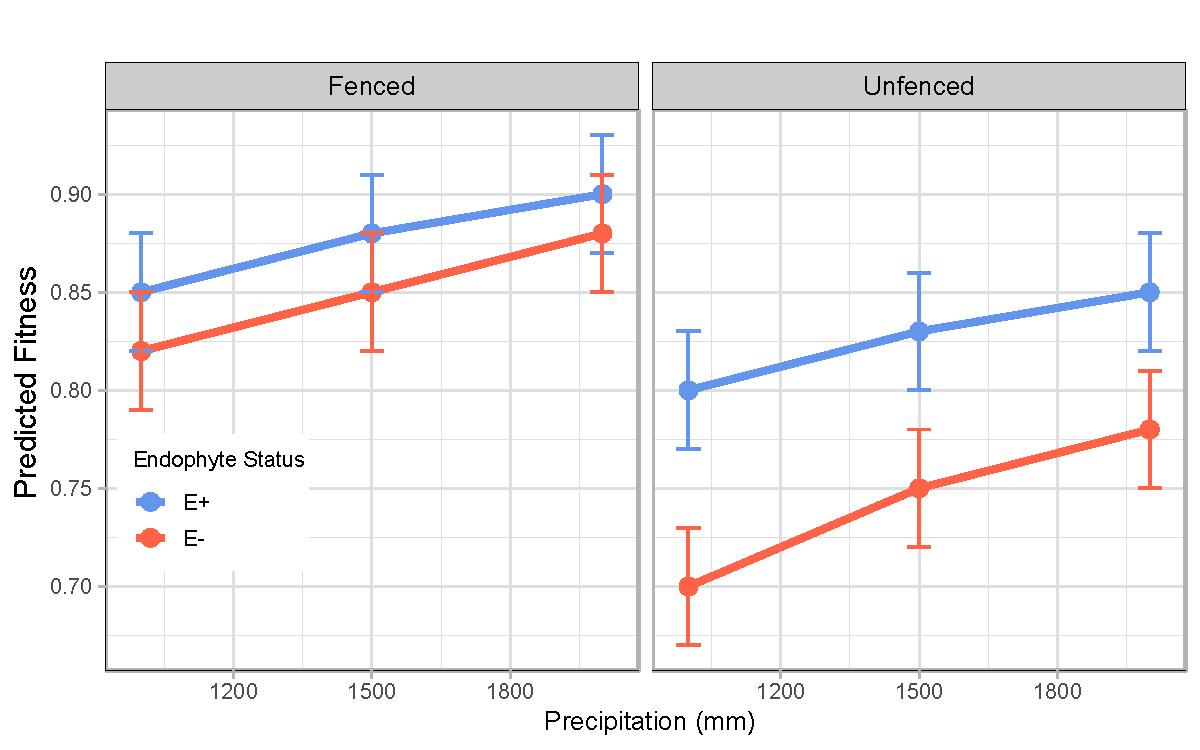
\includegraphics[width=1\textwidth]{../Figure/Prediction.pdf}
    \caption{Conceptual framework illustrating the predicted effects of abiotic stress, biotic stress, and endophyte-mediated mutualism on host plant fitness (adapted from \citep{porter2020beneficial}). 
    (a) \textbf{Endophyte-driven stress amelioration scenario:} Endophytes are predicted to enhance host performance under increasing abiotic stress (e.g., low precipitation) in the absence of herbivores by mitigating drought-related physiological costs. 
    %Abiotic stress is the primary driver of host fitness, and endophyte-mediated benefits become more pronounced as stress intensifies. 
    (b) \textbf{Reduced endophyte-mediated benefits scenario:} When abiotic stress is combined with herbivory, the positive effect of endophytes is expected to weaken. Limited plant resources are divided between defense against herbivores and sustaining the endophyte, reducing the endophyte’s capacity to ameliorate drought stress and potentially resulting in a net cost of hosting an endophyte. 
    Colors are used solely for visualization: blue lines represent endophyte-infected plants and violet lines represent endophyte-free plants.}
    \label{fig:prediction}
\end{figure}


\clearpage
{
\captionsetup[figure]{list=no}
\begin{figure}[h]
\centering
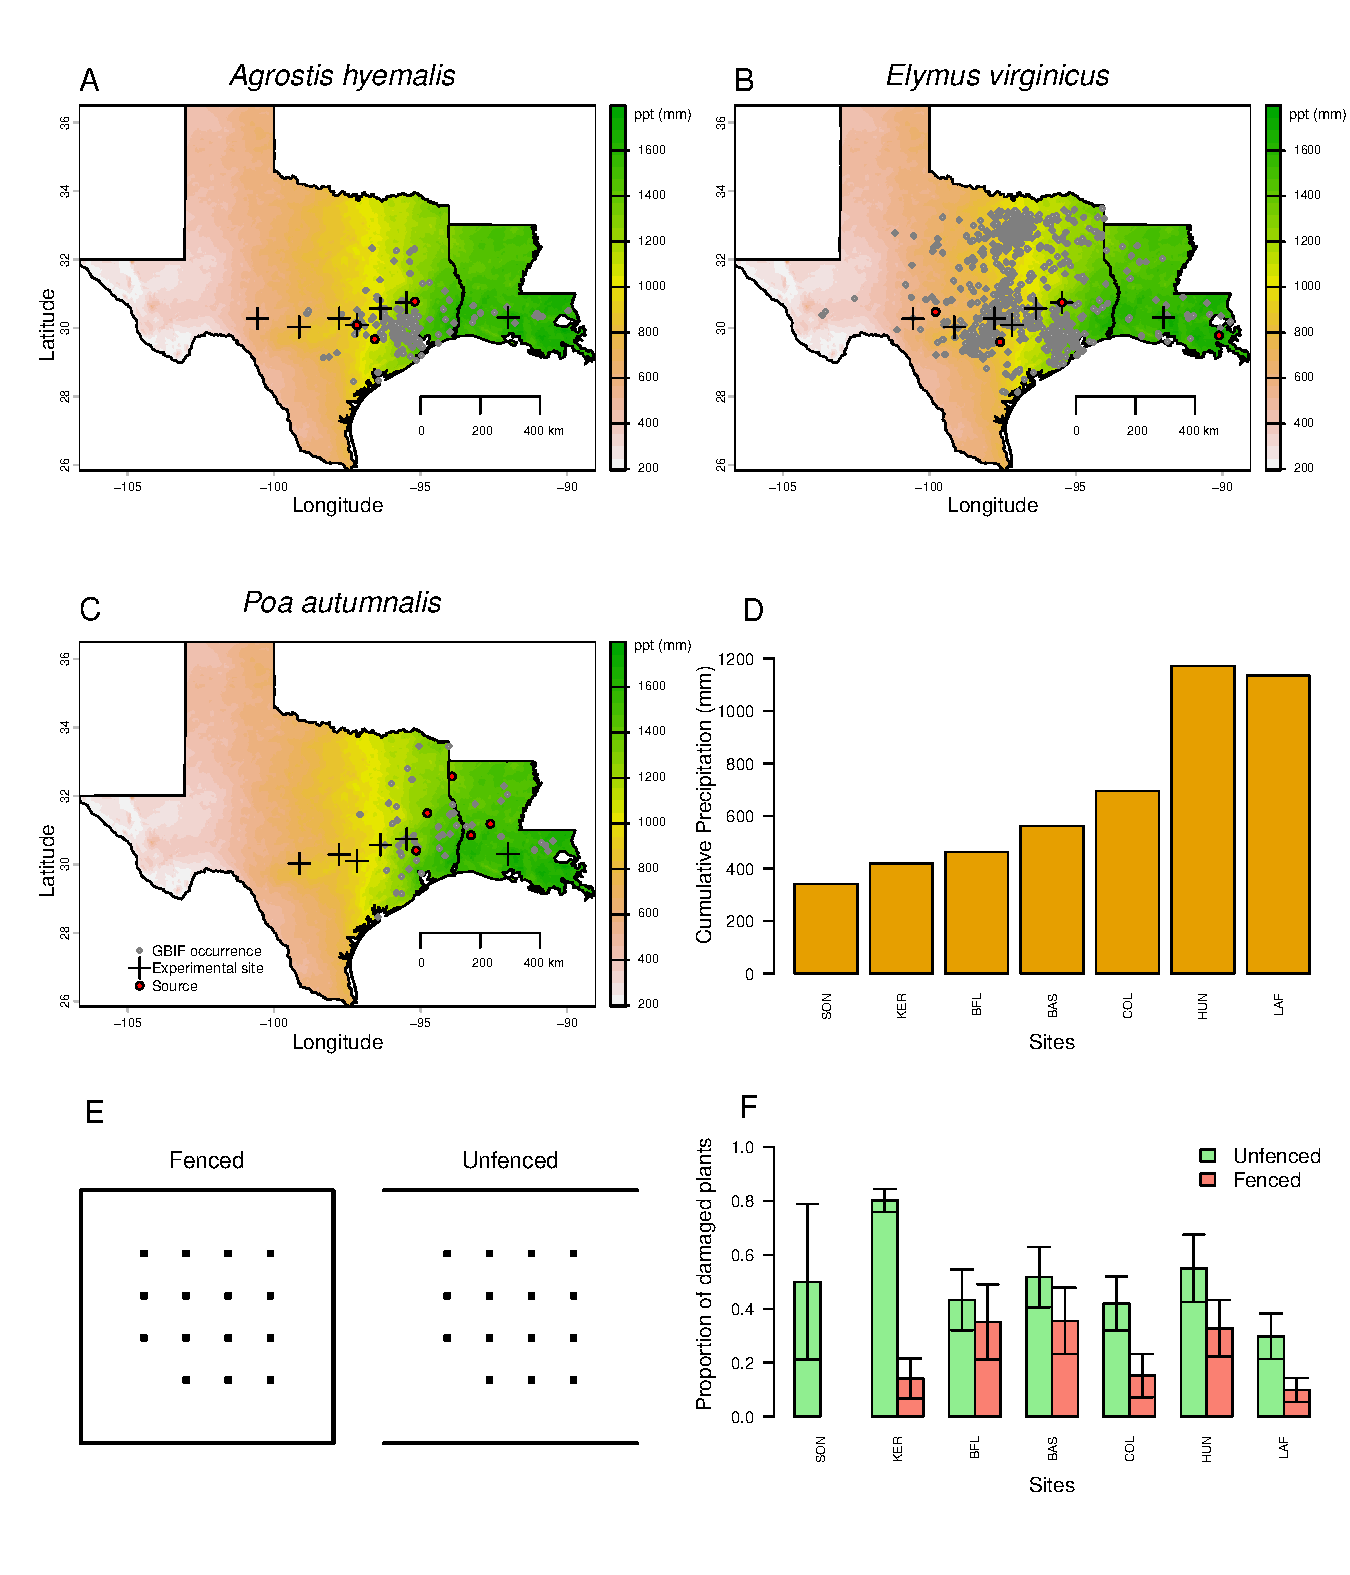
\includegraphics[width=0.92\textwidth]{../Figure/clim_map.pdf}
\caption{Distribution of common garden sites along a natural aridity gradient from Texas to Louisiana, US for (A) \emph{Agrostis hyemalis}, (B) \emph{Elymus virginicus}, and (C) \emph{Poa autumnalis}. 
Climate data in A–C are based on 30-year normals of climate predictions (1996–2025) from PRISM data \citep{PRISM2024}, illustrating the precipitation gradient across experimental sites (scale on the right is in mm). 
Red dots indicate the locations of source populations, while grey dots represent Global Biodiversity Information Facility (GBIF) occurrence records for each species within the study area \citep{gbif2025_aghy,gbif2025_elvi,gbif2025_poau}.
(D) Annual cumulative precipitation during each census year (May 2023 – June 2025) at each experimental site, ordered west to east. 
Values are also derived from PRISM climate data.
(E) Schematic illustration of fenced (left) and unfenced (right) plots used to assess herbivory. 
Symbols (+/$-$) represent plant endophyte status, with ``+'' indicating endophyte-positive and ``$-$'' indicating endophyte-free individuals; plot shape corresponds to experimental design.
(F) Proportion of damaged plants in fenced (salmon) and unfenced (light green) plots across experimental sites, with mean ± standard error. 
Sites are ordered west to east as in panel D. 
Panels E–F illustrate herbivory treatments and outcomes, and species-specific breakdowns are provided in Supplementary Figures.}
\label{fig:site}
\end{figure}
}
\clearpage

{
\captionsetup[figure]{list=no}
\begin{figure}[H]
\centering
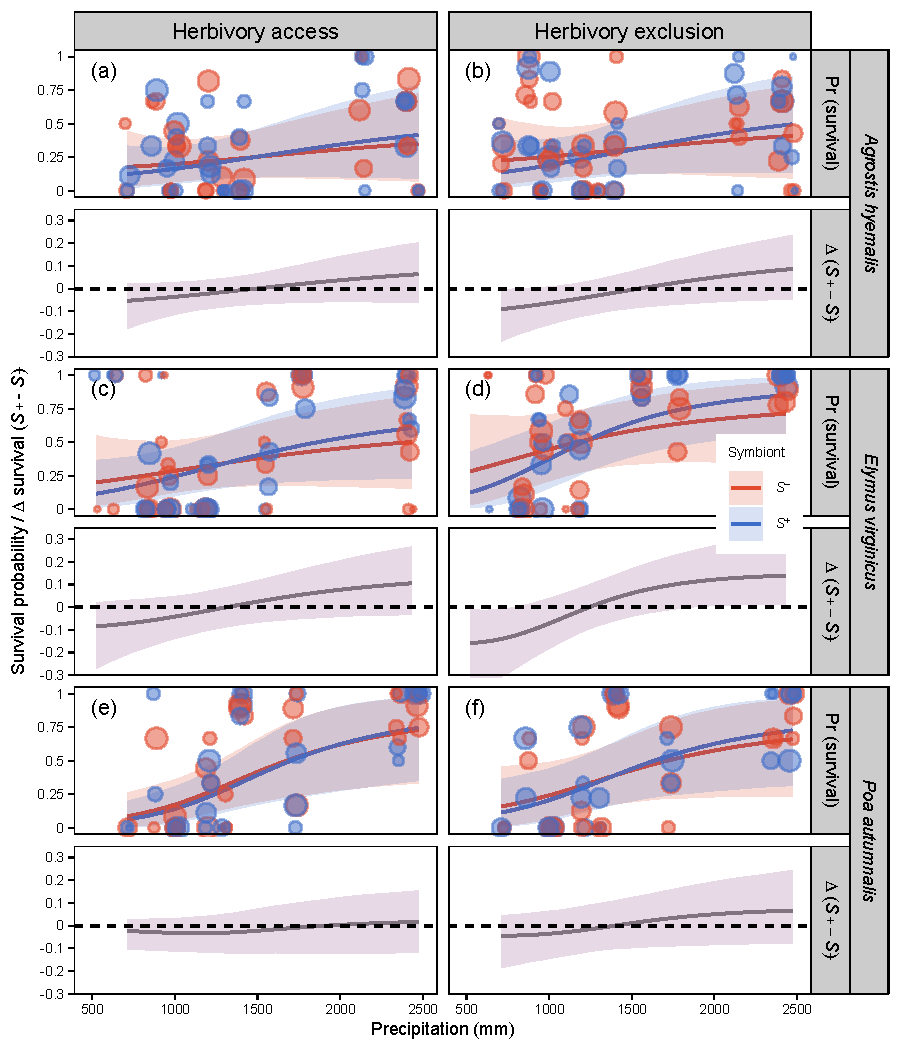
\includegraphics[width=1\textwidth]{../Figure/PrSurvival_diff.pdf}
\caption{Predicted survival rate (top panels) and endophyte effect (\(\Delta = \mathrm{E^+ - E^-}\), bottom panels) across precipitation gradients. 
Lines show posterior means for E\(^+\) (blue) and E\(^-\) (red), with shading indicating 90\% credible intervals. 
Points represent mean observed survival per plot,  jittered  for visualization.  
The dashed line at \(\Delta = 0\) indicates no endophyte effect. 
Panels are organized by species and herbivory treatment (Fenced, Unfenced).}
\label{fig:Surv}
\end{figure}
}

{
\captionsetup[figure]{list=no}
\begin{figure}[H]
\centering
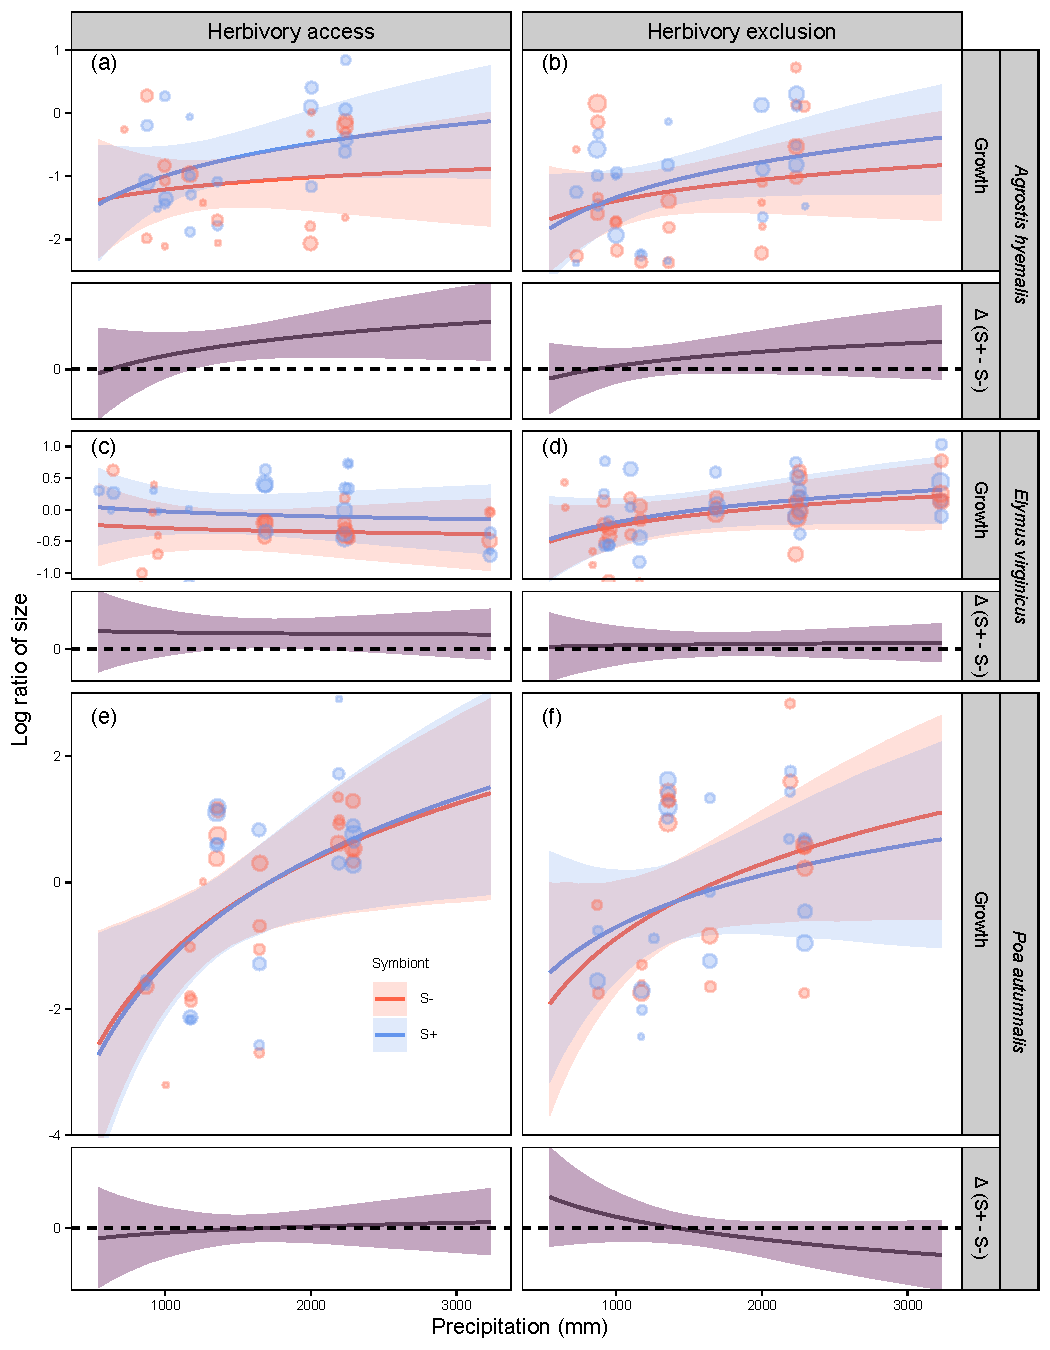
\includegraphics[width=1\textwidth]{../Figure/Growth_diff.pdf}
\caption{Predicted relative growth from year to the next year (top panels) and endophyte effect (\(\Delta = \mathrm{E^+ - E^-}\), bottom panels) across precipitation gradients. 
Lines show posterior means for E\(^+\) (blue) and E\(^-\) (red), with shading indicating 90\% credible intervals. 
Points represent mean observed growth per plot,  jittered  for visualization.  
The dashed line at \(\Delta = 0\) indicates no endophyte effect. 
Panels are organized by species and herbivory treatment (Fenced, Unfenced).}
\label{fig:growth}
\end{figure}
}

{
\captionsetup[figure]{list=no}
\begin{figure}[H]
\centering

\includegraphics[width=1\textwidth]{../Figure/Inflorescence_diff_v.pdf}
\caption{
%Effects of precipitation, endophyte presence, and herbivory on flowering output (number of inflorescences) across three cool-season grass species. 
Predicted number of inflorescences (upper panels) and the difference between endophyte-infected (E$^+$) and endophyte-free (E$^-$) plants ($\Delta$(E$^+$--E$^-$), lower panels) are shown across a gradient of precipitation.
%for \textit{Agrostis hyemalis}, \textit{Elymus virginicus}, and \textit{Poa autumnalis}. 
Shaded areas represent 90\% credible intervals. 
Points indicate observed means, jittered  for visualization. 
Panels are grouped by species and herbivory treatment (Fenced, Unfenced).}
\label{fig:flowering}
\end{figure}
}
\clearpage

\captionsetup[figure]{list=no}
\begin{figure}[H]
\centering
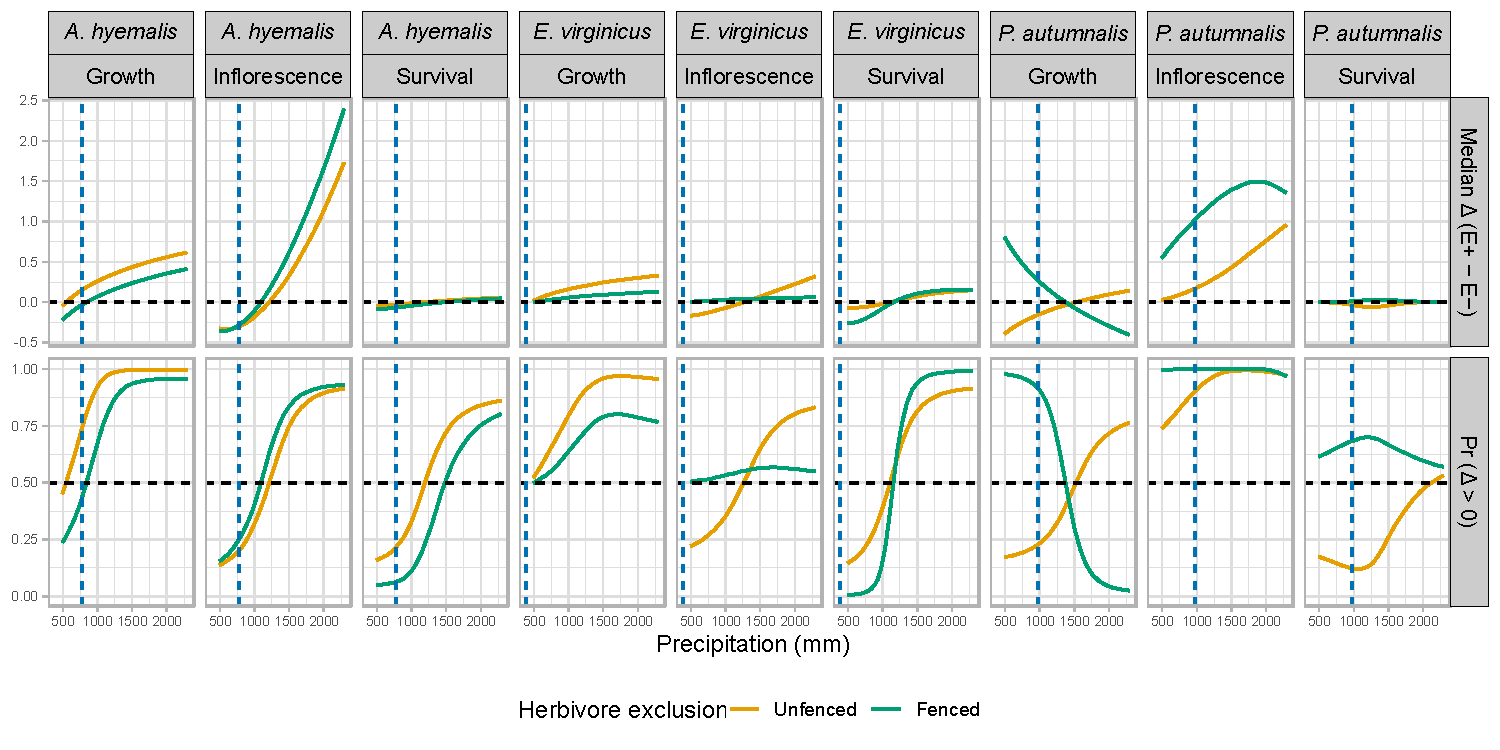
\includegraphics[width=1\textwidth]{../Figure/All_traits_diff_stat.pdf}
\caption{
Predicted effects of herbivore exclusion on survival, growth, and inflorescence production across precipitation gradients for \textit{A. hyemalis}, \textit{E. virginicus}, and \textit{P. autumnalis}. Panels show the median difference between fenced and unfenced treatments ($\Delta = E^{+} - E^{-}$) and the probability that this difference is positive ($\Pr[\Delta > 0]$). Horizontal dashed lines indicate $\Delta = 0$ and $\Pr(\Delta > 0) = 0.5$, and vertical dashed lines denote species-specific mean annual precipitation at range limits. Colors indicate herbivore exclusion treatments.
}
\label{fig:allstat}
\end{figure}
}
\clearpage

\section*{Tables}
{
\captionsetup[table]{list=no}

\begin{table}[h]
\centering
\caption{Comparison of models assessing the drivers of grass--endophyte symbiosis across four fitness components (vital rates). 
$\Delta$ELPD represents the difference in expected log predictive density relative to the best-fitting model, and SE denotes the standard error of this difference.}
\begin{tabular}{lllrr}
\toprule
\textbf{Vital rate} & \textbf{Model type} & & \textbf{$\Delta$ELPD} & \textbf{SE} \\
\midrule
Survival      & Endophyte $\times$ Climate                     & & 0.00   & 0.00 \\
              & Endophyte $\times$ Herbivory                   & & $-4.65$ & 2.05 \\
              & Endophyte $\times$ Climate $\times$ Herbivory  & & $-5.23$ & 3.82 \\
Growth        & Endophyte $\times$ Climate                     & & 0.00   & 0.00 \\
              & Endophyte $\times$ Herbivory                   & & $-0.27$ & 3.24 \\
              & Endophyte $\times$ Climate $\times$ Herbivory  & & $-0.31$ & 3.51 \\
Inflorescence & Endophyte $\times$ Climate                     & & 0.00   & 0.00 \\
              & Endophyte $\times$ Herbivory                   & & $-0.74$ & 2.70 \\
              & Endophyte $\times$ Climate $\times$ Herbivory  & & $-0.90$ & 3.39 \\
Spikelet      & Endophyte $\times$ Climate                     & & 0.00   & 0.00 \\
              & Endophyte $\times$ Herbivory                   & & $-0.92$ & 3.31 \\
              & Endophyte $\times$ Climate $\times$ Herbivory  & & $-3.27$ & 2.44 \\
\bottomrule
\end{tabular}
\label{tab:comp_table_driver}
\end{table}

\clearpage
\appendix

% --- Reset counters ---
\setcounter{figure}{0}
\setcounter{table}{0}
\setcounter{equation}{0}
\setcounter{section}{0}

% --- Section numbering ---
\renewcommand{\thesection}{S.\arabic{section}}

% --- Equation numbering ---
\renewcommand{\theequation}{S\arabic{equation}}

% --- Figure numbering ---
\renewcommand{\figurename}{Fig}       % replaces "Figure" with "Fig"
\renewcommand{\thefigure}{S\arabic{figure}}  % just add S before the number


%\renewcommand{\figurename}{Figure}  % ensures it prints "Figure S1"

% --- Table numbering ---
\renewcommand{\thetable}{S\arabic{table}}
\renewcommand{\tablename}{Table}    % ensures it prints "Table S1"

\section{Supporting Information}
% Page with only list of supplementary figures and tables
%\listoffigures
%\clearpage
%\listoftables
%\clearpage

\subsection{Supporting Methods}
\subsection*{Candidate models for abiotic and biotic drivers of cool-season grass species} \label{sec:models}
\begin{enumerate}
    \item \textbf{Endophyte × Climate model:} includes endophyte status ($\text{endo}$), precipitation ($P$), and their interaction:
    \begin{align*}
    \mu_i &= \beta_0[\text{Sp}_i] + \beta_{\text{endo}}[\text{Sp}_i]\,endo_i + \beta_P[\text{Sp}_i] P_i 
            + \beta_{\text{endo}\times P}[\text{Sp}_i]\,endo_i P_i \\
    &\quad + \phi_{\text{site}[i],\text{Sp}_i} + \omega_{\text{source}[i],\text{Sp}_i} + \rho_{\text{plot}[i],\text{Sp}_i}
    \end{align*}

    \item \textbf{Endophyte × Herbivory model:} includes endophyte status ($\text{endo}$), herbivory ($\text{herb}$), and their interaction:
    \begin{align*}
    \mu_i &= \beta_0[\text{Sp}_i] + \beta_{\text{endo}}[\text{Sp}_i]\,endo_i + \beta_{\text{herb}}[\text{Sp}_i]\,herb_i 
            + \beta_{\text{endo}\times \text{herb}}[\text{Sp}_i]\,endo_i\,herb_i \\
    &\quad + \phi_{\text{site}[i],\text{Sp}_i} + \omega_{\text{source}[i],\text{Sp}_i} + \rho_{\text{plot}[i],\text{Sp}_i}
    \end{align*}

    \item \textbf{Endophyte × Climate × Herbivory:} combines all predictors and interactions up to the three-way interaction:
    \begin{align*}
    \mu_i &= \beta_0[\text{Sp}_i] + \beta_P[\text{Sp}_i] P_i + \beta_{\text{endo}}[\text{Sp}_i]\,endo_i + \beta_{\text{herb}}[\text{Sp}_i]\,herb_i \\
    &\quad + \beta_{\text{endo}\times P}[\text{Sp}_i]\,endo_i P_i 
          + \beta_{\text{herb}\times P}[\text{Sp}_i]\,herb_i P_i
          + \beta_{\text{herb}\times \text{endo}}[\text{Sp}_i]\,herb_i\,endo_i \\
    &\quad + \beta_{\text{endo}\times \text{herb} \times P}[\text{Sp}_i]\,endo_i\,herb_i\,P_i
          + \phi_{\text{site}[i],\text{Sp}_i} + \omega_{\text{source}[i],\text{Sp}_i} + \rho_{\text{plot}[i],\text{Sp}_i}
    \end{align*}
\end{enumerate}

In these models, the $\beta$ coefficients represent species-specific effects. 
The intercept $\beta_0[\text{Sp}_i]$ corresponds to the baseline value of the vital rate for species $\text{Sp}_i$ in the absence of predictors. $\beta_{\text{endo}}[\text{Sp}_i]$ and $\beta_{\text{herb}}[\text{Sp}_i]$ describe the effects of endophyte presence and herbivory, respectively. The linear effect of precipitation is captured by $\beta_P[\text{Sp}_i]$, while interactions are represented by $\beta_{\text{endo}\times P}[\text{Sp}_i]$, $\beta_{\text{herb}\times P}[\text{Sp}_i]$, $\beta_{\text{endo}\times \text{herb}}[\text{Sp}_i]$, and the three-way interaction $\beta_{\text{endo}\times \text{herb} \times P}[\text{Sp}_i]$. 
All models include hierarchical random effects for site-year, source population, and plot, with species-specific random effects $\phi_{\text{site}[i],\text{Sp}_i} \sim \mathcal{N}(0, \sigma_{\text{site}})$, $\omega_{\text{source}[i],\text{Sp}_i} \sim \mathcal{N}(0, \sigma_{\text{source}})$, and $\rho_{\text{plot}[i],\text{Sp}_i} \sim \mathcal{N}(0, \sigma_{\text{plot}})$.
\clearpage 

\subsection{Supporting Tables}
\begin{table}[ht]
\centering
\caption[Geographic coordinates and descriptions of source populations for study species]{Geographic coordinates and brief descriptions of source populations for \textit{Agrostis hyemalis} (AGHY), \textit{Elymus virginicus} (ELVI), and \textit{Poa autumnalis} (POAU).}
\label{tab:source_pop}
%\begin{tabular}{lllll}
\begin{tabular}{llrrp{6cm}}
\toprule
\textbf{Species} & \textbf{Population} & \textbf{Latitude} & \textbf{Longitude} & \textbf{Description} \\
\midrule
AGHY & SJC  & 30.771969 & -95.200620 & San Jacinto County, TX \\
AGHY & COHR & 29.672833 & -96.567517 & Columbus, TX \\
AGHY & LPEF & 30.085383 & -97.172508 & Lost Pines \\
POAU & LA7  & 30.849660 & -93.276772 & DeRidder, LA \\
POAU & LA1  & 32.568125 & -93.932976 & \tom{Jean Lafitte National Historical Park and Preserve}{Double check this. There were no POAU collected from Jean Lafitte Park.} \\
POAU & LA2  & 31.183040 & -92.616969 & Jean Lafitte National Historical Park and Preserve \\
POAU & SFAEF & 31.492158 & -94.772200 & Stephen F. Austin Experimental Forest, TX \\
POAU & WB   & 30.399346 & -95.150026 & Sam Houston National Forest \\
ELVI & HUNT & 30.741797 & -95.474508 & Sam Houston State University Field Station \\
ELVI & \tom{SHS}{This row is exactly redundant with the previous row, it just has a different population name.}  & 30.741797 & -95.474508 & Sam Houston State University Field Station \\
ELVI & RL5  & 30.471717 & -99.783803 & Texas Tech University Field Station, Junction \\
ELVI & PALM & 29.591623 & -97.584781 & Palmetto State Park, TX \\
ELVI & JLP  & 29.785105 & -90.114933 & Jean Lafitte Park, outside of New Orleans \\
\bottomrule
\end{tabular}
\end{table}
\clearpage  % forces the next figure to start on a new page

\begin{table}[ht]
\caption[Geographic coordinates of common garden sites for study species]{Common garden sites used for reciprocal transplant and environmental manipulation studies.}
\label{tab:exp_sites}
\begin{tabular}{llrr}
\hline
\textbf{Site} & \textbf{Code} & \textbf{Latitude} & \textbf{Longitude} \\
\hline
University of Louisiana Ecology Center & LAF & 30.304773 & -92.012401 \\
Center for Biological Field Studies & HUN & 30.742815 & -95.476881 \\
TAMU Ecology and Natural Resource Teaching Area & COL & 30.569302 & -96.366324 \\
UT Stengl Lost Pines Field Station & BAS & 30.092343 & -97.172442 \\
Private property in Kerrville, TX & KER & 30.028437 & -99.142888 \\
Brackenridge Field Laboratory & BFL & 30.284866 & -97.780675 \\
TAMU Sonora Station & SON & 30.273467 & -100.561463 \\
\hline
\end{tabular}
\end{table}
\clearpage 

\begin{table}[h]
\centering
\caption{Realized numbers of endophyte-free (E$-$) and endophyte-infected (E$+$) individuals per species and population, with total number of clones.}
\begin{tabular}{llrrr}
\toprule
\textbf{Species} & \textbf{Population} & \textbf{E$-$} & \textbf{E$+$} & \textbf{Total clones} \\
\midrule
\textit{Agrostis hyemalis} & COHR  & 238 & 242 & 480 \\
\textit{Agrostis hyemalis} & LPEF  & 227 & 236 & 463 \\
\textit{Agrostis hyemalis} & SJC   & 232 & 225 & 457 \\
\textit{Elymus virginicus} & HUNT  & 89  & 19  & 108 \\
\textit{Elymus virginicus} & JLP   & 156 & 135 & 291 \\
\textit{Elymus virginicus} & PALM  & 319 & 423 & 742 \\
\textit{Elymus virginicus} & RL5   & 141 & 81  & 222 \\
\textit{Elymus virginicus} & SHS   & 1   & 49  & 50  \\
\textit{Poa autumnalis}     & LA1   & 119 & 101 & 220 \\
\textit{Poa autumnalis}     & LA2   & 201 & 233 & 434 \\
\textit{Poa autumnalis}     & LA7   & 89  & 72  & 161 \\
\textit{Poa autumnalis}     & SFAEF & 207 & 212 & 419 \\
\bottomrule
\end{tabular}
\label{tab:endo_counts}
\end{table}

\clearpage

\begin{table}[ht]
\centering
\caption[Model comparison for vital rates (quadratic vs. linear models)]{Comparison of candidate models (quadratic vs. linear) for each vital rate based on leave-one-out cross-validation (LOOCV). 
ELPD difference is relative to the best model.}
\label{tab:model_comparison}
\begin{tabular}{l l r r}
\hline
\textbf{Vital rate} & \textbf{Model type} & \textbf{ELPD difference} & \textbf{SE difference} \\
\hline
Survival        & Quadratic & 0       & 0.00 \\
Survival        & Linear    & -0.055  & 1.09 \\
Growth          & Quadratic & 0       & 0.00 \\
Growth          & Linear    & -0.187  & 1.33 \\
Inflorescence   & Quadratic & 0       & 0.00 \\
Inflorescence   & Linear    & -1.510  & 1.43 \\
Spikelet        & Quadratic & 0       & 0.00 \\
Spikelet        & Linear    & -0.849  & 1.32 \\
\hline
\end{tabular}
\end{table}
\clearpage
 
 \begin{landscape}
\begin{table}[ht]
\centering
\caption{Posterior summary of survival ratios (E$^+$ / E$^-$) under low-climate stress. Median, 90\% credible intervals, and posterior probability that E$^+$ performs worse than E$^-$ are shown for each species and herbivory treatment.}
\label{tab:ratio_surv_summary}
\begin{tabular}{llrrrrr}
\hline
Species & Herbivory & Median ratio & Lower 90\% & Upper 90\% & Prob(E$^+$ worse) \\
\hline
Agrostis hyemalis & Herbivory access & 0.666 & 0.253 & 1.36 & 0.825 \\
Agrostis hyemalis & Herbivory exclusion & 0.544 & 0.221 & 1.01 & 0.946 \\
Elymus virginicus & Herbivory access & 0.602 & 0.202 & 1.44 & 0.831 \\
Elymus virginicus & Herbivory exclusion & 0.352 & 0.0975 & 0.801 & 0.991 \\
Poa autumnalis & Herbivory access & 0.405 & 0.0785 & 1.83 & 0.837 \\
Poa autumnalis & Herbivory exclusion & 1.28 & 0.356 & 4.91 & 0.371 \\
\hline
\end{tabular}
\end{table}
\end{landscape}
\clearpage  % forces the next figure to start on a new page


\begin{landscape}
\begin{table}[ht]
\centering
\small
\caption[Summaries of $\Delta$ (E$^{+}$ $-$ E$^{-}$) for survival across precipitation bins]{
Posterior summaries of $\Delta$ (E$^{+}$ $-$ E$^{-}$) for survival across precipitation quartiles for each species and herbivore treatment. 
Median, 90\% credible interval, and posterior probability that $\Delta > 0$ are shown. 
Herbivore exclusion: Fenced = herbivores excluded, Unfenced = herbivores had access.
}
\label{tab:delta_summary_surv_quantiles}
\begin{tabular}{llrrrrr}
\hline
\textbf{Species} & \textbf{Herbivore treatment} & \textbf{Precipitation bin (mm)} & \textbf{Median $\Delta$} & \textbf{Lower 90\%} & \textbf{Upper 90\%} & \textbf{P($\Delta>0$)} \\
\hline
\textit{Agrostis hyemalis} & Herbivory access    & 493  & -0.049 & -0.302 & 0.053 & 0.158 \\
\textit{Agrostis hyemalis} & Herbivory access    & 678  & -0.038 & -0.215 & 0.052 & 0.187 \\
\textit{Agrostis hyemalis} & Herbivory access    & 1036 & -0.012 & -0.099 & 0.058 & 0.357 \\
\textit{Agrostis hyemalis} & Herbivory access    & 1424 & 0.015  & -0.050 & 0.102 & 0.681 \\
\textit{Agrostis hyemalis} & Herbivory access    & 2294 & 0.056  & -0.035 & 0.249 & 0.860 \\
\textit{Agrostis hyemalis} & Herbivory exclusion & 493  & -0.090 & -0.358 & 0.000 & 0.051 \\
\textit{Agrostis hyemalis} & Herbivory exclusion & 678  & -0.076 & -0.264 & 0.002 & 0.057 \\
\textit{Agrostis hyemalis} & Herbivory exclusion & 1036 & -0.041 & -0.142 & 0.019 & 0.127 \\
\textit{Agrostis hyemalis} & Herbivory exclusion & 1424 & -0.004 & -0.085 & 0.072 & 0.448 \\
\textit{Agrostis hyemalis} & Herbivory exclusion & 2294 & 0.047  & -0.052 & 0.224 & 0.802 \\
\textit{Elymus virginicus} & Herbivory access    & 493  & -0.069 & -0.321 & 0.050 & 0.145 \\
\textit{Elymus virginicus} & Herbivory access    & 678  & -0.065 & -0.254 & 0.068 & 0.189 \\
\textit{Elymus virginicus} & Herbivory access    & 1036 & -0.014 & -0.143 & 0.113 & 0.424 \\
\textit{Elymus virginicus} & Herbivory access    & 1424 & 0.061  & -0.069 & 0.194 & 0.779 \\
\textit{Elymus virginicus} & Herbivory access    & 2294 & 0.148  & -0.031 & 0.356 & 0.914 \\
\textit{Elymus virginicus} & Herbivory exclusion & 493  & -0.259 & -0.550 & -0.058 & 0.006 \\
\textit{Elymus virginicus} & Herbivory exclusion & 678  & -0.230 & -0.430 & -0.058 & 0.012 \\
\textit{Elymus virginicus} & Herbivory exclusion & 1036 & -0.059 & -0.183 & 0.061  & 0.210 \\
\textit{Elymus virginicus} & Herbivory exclusion & 1424 & 0.090  & -0.022 & 0.225  & 0.907 \\
\textit{Elymus virginicus} & Herbivory exclusion & 2294 & 0.154  & 0.031  & 0.400  & 0.992 \\
\textit{Poa autumnalis}    & Herbivory access    & 493  & -0.001 & -0.101 & 0.005  & 0.175 \\
\textit{Poa autumnalis}    & Herbivory access    & 678  & -0.005 & -0.143 & 0.010  & 0.154 \\
\textit{Poa autumnalis}    & Herbivory access    & 1036 & -0.043 & -0.196 & 0.022  & 0.118 \\
\textit{Poa autumnalis}    & Herbivory access    & 1424 & -0.051 & -0.188 & 0.060  & 0.214 \\
\textit{Poa autumnalis}    & Herbivory access    & 2294 & 0.000  & -0.124 & 0.137  & 0.532 \\
\textit{Poa autumnalis}    & Herbivory exclusion & 493  & 0.000  & -0.019 & 0.067  & 0.614 \\
\textit{Poa autumnalis}    & Herbivory exclusion & 678  & 0.001  & -0.033 & 0.092  & 0.641 \\
\textit{Poa autumnalis}    & Herbivory exclusion & 1036 & 0.016  & -0.058 & 0.136  & 0.689 \\
\textit{Poa autumnalis}    & Herbivory exclusion & 1424 & 0.029  & -0.088 & 0.166  & 0.679 \\
\textit{Poa autumnalis}    & Herbivory exclusion & 2294 & 0.002  & -0.117 & 0.151  & 0.570 \\
\hline
\end{tabular}
\end{table}
\end{landscape}
\clearpage

\begin{landscape}
\begin{table}[ht]
\centering
\small
\caption[Summaries of $\Delta$ (E$^{+}$ $-$ E$^{-}$) for growth across precipitation quantiles]{Posterior summaries of $\Delta$ (E$^{+}$ $-$ E$^{-}$) for growth across precipitation quantiles for each species and herbivore treatment. 
Positive median values indicate beneficial effects of endophytes; negative medians indicate costly effects.}
\label{tab:delta_summary_grow}
\begin{tabular}{llrrrrr}
\hline
\textbf{Species} & \textbf{Herbivore treatment} & \textbf{Precipitation (mm)} & \textbf{Median $\Delta$} & \textbf{Lower 90\%} & \textbf{Upper 90\%} & \textbf{P($\Delta>0$)} \\
\hline
\textit{Agrostis hyemalis} & Herbivory access    & 493  & -0.046 & -0.643 & 0.561 & 0.450 \\
\textit{Agrostis hyemalis} & Herbivory access    & 678  & 0.092  & -0.352 & 0.543 & 0.629 \\
\textit{Agrostis hyemalis} & Herbivory access    & 1036 & 0.274  & -0.019 & 0.571 & 0.939 \\
\textit{Agrostis hyemalis} & Herbivory access    & 1424 & 0.412  & 0.147  & 0.683 & 0.994 \\
\textit{Agrostis hyemalis} & Herbivory access    & 2294 & 0.616  & 0.212  & 1.022 & 0.994 \\
\textit{Agrostis hyemalis} & Herbivory exclusion & 493  & -0.221 & -0.723 & 0.290 & 0.237 \\
\textit{Agrostis hyemalis} & Herbivory exclusion & 678  & -0.090 & -0.466 & 0.284 & 0.347 \\
\textit{Agrostis hyemalis} & Herbivory exclusion & 1036 & 0.084  & -0.165 & 0.336 & 0.710 \\
\textit{Agrostis hyemalis} & Herbivory exclusion & 1424 & 0.214  & -0.034 & 0.460 & 0.925 \\
\textit{Agrostis hyemalis} & Herbivory exclusion & 2294 & 0.411  & 0.017  & 0.799 & 0.956 \\
\textit{Elymus virginicus} & Herbivory access    & 493  & 0.017  & -0.618 & 0.647 & 0.520 \\
\textit{Elymus virginicus} & Herbivory access    & 678  & 0.084  & -0.400 & 0.566 & 0.614 \\
\textit{Elymus virginicus} & Herbivory access    & 1036 & 0.168  & -0.137 & 0.476 & 0.814 \\
\textit{Elymus virginicus} & Herbivory access    & 1424 & 0.232  & -0.002 & 0.470 & 0.948 \\
\textit{Elymus virginicus} & Herbivory access    & 2294 & 0.330  & 0.008  & 0.643 & 0.955 \\
\textit{Elymus virginicus} & Herbivory exclusion & 493  & -0.002 & -0.594 & 0.578 & 0.498 \\
\textit{Elymus virginicus} & Herbivory exclusion & 678  & 0.023  & -0.419 & 0.457 & 0.532 \\
\textit{Elymus virginicus} & Herbivory exclusion & 1036 & 0.060  & -0.205 & 0.316 & 0.651 \\
\textit{Elymus virginicus} & Herbivory exclusion & 1424 & 0.087  & -0.101 & 0.274 & 0.777 \\
\textit{Elymus virginicus} & Herbivory exclusion & 2294 & 0.130  & -0.160 & 0.410 & 0.767 \\
\textit{Poa autumnalis}    & Herbivory access    & 493  & -0.393 & -1.089 & 0.289 & 0.174 \\
\textit{Poa autumnalis}    & Herbivory access    & 678  & -0.283 & -0.803 & 0.230 & 0.185 \\
\textit{Poa autumnalis}    & Herbivory access    & 1036 & -0.136 & -0.448 & 0.179 & 0.242 \\
\textit{Poa autumnalis}    & Herbivory access    & 1424 & -0.024 & -0.245 & 0.202 & 0.431 \\
\textit{Poa autumnalis}    & Herbivory access    & 2294 & 0.143  & -0.175 & 0.474 & 0.763 \\
\textit{Poa autumnalis}    & Herbivory exclusion & 493  & 0.806  & 0.137  & 1.478 & 0.977 \\
\textit{Poa autumnalis}    & Herbivory exclusion & 678  & 0.556  & 0.058  & 1.060 & 0.967 \\
\textit{Poa autumnalis}    & Herbivory exclusion & 1036 & 0.223  & -0.077 & 0.529 & 0.890 \\
\textit{Poa autumnalis}    & Herbivory exclusion & 1424 & -0.028 & -0.251 & 0.199 & 0.418 \\
\textit{Poa autumnalis}    & Herbivory exclusion & 2294 & -0.406 & -0.737 & -0.067 & 0.025 \\
\hline

\end{tabular}
\end{table}
\end{landscape}
\clearpage

\begin{landscape}
\begin{table}[ht]
\centering
\caption[Summaries of $\Delta$ (E$^{+}$ $-$ E$^{-}$) for inflorescences across precipitation quantiles]{Posterior summaries of $\Delta$ (E$^{+}$ $-$ E$^{-}$) for flowering output at precipitation quantiles for each species and herbivore  treatment. 
Median, 90\% credible interval, and posterior probability that $\Delta > 0$ are shown. 
Herbivore exclusion: Fenced = herbivores excluded, Unfenced = herbivores had access.}
\label{tab:delta_summary_flow}
\begin{tabular}{llrrrrr}
\hline
Species & Herbivore treatment & Precipitation (mm) & Median $\Delta$  & Lower 90\% & Upper 90\% & P($\Delta>0$) \\
\hline
Species & Herbivory & Precipitation (mm) & Median $\Delta$  & Lower 90\% & Upper 90\% & P($\Delta>0$) \\
\hline
\textit{Agrostis hyemalis} & Herbivory access    & 493  & -0.325 & -1.371 & 0.229  & 0.137 \\
\textit{Agrostis hyemalis} & Herbivory access    & 678  & -0.327 & -1.230 & 0.320  & 0.172 \\
\textit{Agrostis hyemalis} & Herbivory access    & 1036 & -0.157 & -0.929 & 0.557  & 0.344 \\
\textit{Agrostis hyemalis} & Herbivory access    & 1424 & 0.231  & -0.589 & 1.219  & 0.691 \\
\textit{Agrostis hyemalis} & Herbivory access    & 2294 & 1.730  & -0.289 & 6.251  & 0.914 \\
\textit{Agrostis hyemalis} & Herbivory exclusion & 493  & -0.355 & -1.550 & 0.311  & 0.154 \\
\textit{Agrostis hyemalis} & Herbivory exclusion & 678  & -0.332 & -1.339 & 0.426  & 0.206 \\
\textit{Agrostis hyemalis} & Herbivory exclusion & 1036 & -0.067 & -0.897 & 0.796  & 0.439 \\
\textit{Agrostis hyemalis} & Herbivory exclusion & 1424 & 0.481  & -0.492 & 1.772  & 0.800 \\
\textit{Agrostis hyemalis} & Herbivory exclusion & 2294 & 2.394  & -0.264 & 8.520  & 0.930 \\
\textit{Elymus virginicus} & Herbivory access    & 493  & -0.167 & -0.742 & 0.249  & 0.220 \\
\textit{Elymus virginicus} & Herbivory access    & 678  & -0.142 & -0.606 & 0.255  & 0.250 \\
\textit{Elymus virginicus} & Herbivory access    & 1036 & -0.062 & -0.410 & 0.274  & 0.369 \\
\textit{Elymus virginicus} & Herbivory access    & 1424 & 0.046  & -0.277 & 0.391  & 0.606 \\
\textit{Elymus virginicus} & Herbivory access    & 2294 & 0.320  & -0.226 & 1.141  & 0.831 \\
\textit{Elymus virginicus} & Herbivory exclusion & 493  & 0.006  & -1.001 & 1.434  & 0.505 \\
\textit{Elymus virginicus} & Herbivory exclusion & 678  & 0.015  & -0.824 & 1.125  & 0.512 \\
\textit{Elymus virginicus} & Herbivory exclusion & 1036 & 0.033  & -0.576 & 0.732  & 0.536 \\
\textit{Elymus virginicus} & Herbivory exclusion & 1424 & 0.044  & -0.445 & 0.566  & 0.561 \\
\textit{Elymus virginicus} & Herbivory exclusion & 2294 & 0.064  & -0.808 & 1.089  & 0.551 \\
\textit{Poa autumnalis}    & Herbivory access    & 493  & 0.029  & -0.152 & 1.709  & 0.738 \\
\textit{Poa autumnalis}    & Herbivory access    & 678  & 0.070  & -0.097 & 1.287  & 0.798 \\
\textit{Poa autumnalis}    & Herbivory access    & 1036 & 0.194  & -0.029 & 1.143  & 0.921 \\
\textit{Poa autumnalis}    & Herbivory access    & 1424 & 0.385  & 0.054  & 1.767  & 0.987 \\
\textit{Poa autumnalis}    & Herbivory access    & 2294 & 0.957  & 0.027  & 10.518 & 0.972 \\
\textit{Poa autumnalis}    & Herbivory exclusion & 493  & 0.543  & 0.021  & 14.821 & 0.996 \\
\textit{Poa autumnalis}    & Herbivory exclusion & 678  & 0.744  & 0.072  & 8.201  & 0.998 \\
\textit{Poa autumnalis}    & Herbivory exclusion & 1036 & 1.076  & 0.259  & 4.875  & 1.000 \\
\textit{Poa autumnalis}    & Herbivory exclusion & 1424 & 1.349  & 0.322  & 5.461  & 1.000 \\
\textit{Poa autumnalis}    & Herbivory exclusion & 2294 & 1.355  & 0.031  & 15.437 & 0.968 \\
\hline
\end{tabular}
\end{table}
\end{landscape}

\begin{landscape}
\begin{table}[ht]
\centering
\small
\caption[Summaries of $\Delta$ (E$^{+}$ $-$ E$^{-}$) for inflorescences across precipitation quantiles]{Posterior summaries of $\Delta$ (E$^{+}$ $-$ E$^{-}$) at precipitation quantiles for each species and herbivore  treatment. 
Median, 90\% credible interval, and posterior probability that $\Delta > 0$ are shown. 
Herbivore exclusion: Fenced = herbivores excluded, Unfenced = herbivores had access.}
\label{tab:delta_summary_spike}
\begin{tabular}{llrrrrr}
\hline
Species & Herbivore treatment & Precipitation (mm) & Median $\Delta$  & Lower 90\% & Upper 90\% & P($\Delta>0$) \\
\hline
\textit{Elymus virginicus} & Herbivory access    & 493  & -3.149 & -11.141 & 3.194  & 0.202 \\
\textit{Elymus virginicus} & Herbivory access    & 678  & -2.375 & -8.360  & 2.851  & 0.224 \\
\textit{Elymus virginicus} & Herbivory access    & 1036 & -1.132 & -5.122  & 2.668  & 0.303 \\
\textit{Elymus virginicus} & Herbivory access    & 1424 & -0.095 & -3.238  & 3.106  & 0.481 \\
\textit{Elymus virginicus} & Herbivory access    & 2294 & 1.676  & -2.131  & 6.291  & 0.770 \\
\textit{Elymus virginicus} & Herbivory exclusion & 493  & -4.550 & -11.872 & 1.236  & 0.092 \\
\textit{Elymus virginicus} & Herbivory exclusion & 678  & -3.364 & -8.645  & 1.306  & 0.111 \\
\textit{Elymus virginicus} & Herbivory exclusion & 1036 & -1.444 & -4.572  & 1.644  & 0.211 \\
\textit{Elymus virginicus} & Herbivory exclusion & 1424 & 0.261  & -2.038  & 2.652  & 0.577 \\
\textit{Elymus virginicus} & Herbivory exclusion & 2294 & 3.229  & -0.389  & 8.420  & 0.929 \\
\textit{Poa autumnalis}    & Herbivory access    & 493  & -0.584 & -6.085  & 3.143  & 0.320 \\
\textit{Poa autumnalis}    & Herbivory access    & 678  & -0.584 & -4.893  & 2.756  & 0.330 \\
\textit{Poa autumnalis}    & Herbivory access    & 1036 & -0.408 & -3.240  & 2.226  & 0.373 \\
\textit{Poa autumnalis}    & Herbivory access    & 1424 & -0.025 & -2.094  & 2.056  & 0.491 \\
\textit{Poa autumnalis}    & Herbivory access    & 2294 & 1.097  & -2.362  & 5.455  & 0.719 \\
\textit{Poa autumnalis}    & Herbivory exclusion & 493  & 2.630  & -1.310  & 12.708 & 0.890 \\
\textit{Poa autumnalis}    & Herbivory exclusion & 678  & 2.943  & -0.645  & 10.507 & 0.917 \\
\textit{Poa autumnalis}    & Herbivory exclusion & 1036 & 3.267  & 0.227   & 7.905  & 0.963 \\
\textit{Poa autumnalis}    & Herbivory exclusion & 1424 & 3.333  & 0.797   & 6.547  & 0.987 \\
\textit{Poa autumnalis}    & Herbivory exclusion & 2294 & 2.748  & -1.344  & 8.544  & 0.871 \\
\hline
\end{tabular}
\end{table}
\end{landscape}

%\begin{landscape}
%\begin{table}[ht]
%\centering
%\small
%\caption{Posterior summaries of interaction effects (mean estimate, 95\% credible intervals, and posterior probability) for survival, growth, flowering, and spikelet production across three grass species.}
%\label{tab:interactions}
%\begin{tabular}{l l l r r r r}
%\hline
%Fitness component & Species & Parameter & Estimate & Lower CI & Upper CI & Probability \\
%\hline
%Survival & \textit{Agrostis hyemalis} & Endophyte × Climate & 1.213 & 0.658 & 2.354 & 0.730 \\
%Survival & \textit{Elymus virginicus} & Endophyte × Climate & 1.364 & 0.666 & 2.802 & 0.806 \\
%Survival & \textit{Poa autumnalis} & Endophyte × Climate & 1.255 & 0.483 & 3.344 & 0.681 \\
%Survival & \textit{Agrostis hyemalis} & Endophyte × Herbivory & 0.804 & 0.364 & 1.720 & 0.287 \\
%Survival & \textit{Elymus virginicus} & Endophyte × Herbivory & 0.868 & 0.347 & 2.119 & 0.376 \\
%Survival & \textit{Poa autumnalis} & Endophyte × Herbivory & 1.941 & 0.642 & 6.026 & 0.879 \\
%Survival & \textit{Agrostis hyemalis} & Endophyte × Herbivory × Climate & 1.149 & 0.503 & 2.525 & 0.630 \\
%Survival & \textit{Elymus virginicus} & Endophyte × Herbivory × Climate & 1.450 & 0.560 & 3.880 & 0.774 \\
%Survival & \textit{Poa autumnalis} & Endophyte × Herbivory × Climate & 0.737 & 0.229 & 2.394 & 0.303 \\
%Growth & \textit{Agrostis hyemalis} & Endophyte × Climate & -0.005 & -0.340 & 0.329 & 0.488 \\
%Growth & \textit{Elymus virginicus} & Endophyte × Climate & -0.013 & -0.290 & 0.268 & 0.461 \\
%Growth & \textit{Poa autumnalis} & Endophyte × Climate & 0.208 & -0.156 & 0.559 & 0.873 \\
%Growth & \textit{Agrostis hyemalis} & Endophyte × Herbivory & -0.283 & -0.734 & 0.158 & 0.107 \\
%Growth & \textit{Elymus virginicus} & Endophyte × Herbivory & -0.208 & -0.621 & 0.218 & 0.169 \\
%Growth & \textit{Poa autumnalis} & Endophyte × Herbivory & 0.365 & -0.135 & 0.862 & 0.929 \\
%Growth & \textit{Agrostis hyemalis} & Endophyte × Herbivory × Climate & 0.084 & -0.296 & 0.462 & 0.666 \\
%Growth & \textit{Elymus virginicus} & Endophyte × Herbivory × Climate & 0.060 & -0.296 & 0.405 & 0.634 \\
%Growth & \textit{Poa autumnalis} & Endophyte × Herbivory × Climate & -0.549 & -0.966 & -0.141 & 0.004 \\
%Flowering & \textit{Agrostis hyemalis} & bendoclim & 1.092 & 0.711 & 1.646 & 0.656 \\
%Flowering & \textit{Elymus virginicus} & bendoclim & 1.178 & 0.817 & 1.698 & 0.805 \\
%Flowering & \textit{Poa autumnalis} & bendoclim & 1.103 & 0.725 & 1.689 & 0.676 \\
%Flowering & \textit{Agrostis hyemalis} & bendoherb & 1.014 & 0.577 & 1.784 & 0.523 \\
%Flowering & \textit{Elymus virginicus} & bendoherb & 0.987 & 0.549 & 1.781 & 0.478 \\
%Flowering & \textit{Poa autumnalis} & bendoherb & 1.964 & 1.052 & 3.807 & 0.982 \\
%Flowering & \textit{Agrostis hyemalis} & bendoherbclim & 0.997 & 0.604 & 1.670 & 0.496 \\
%Flowering & \textit{Elymus virginicus} & bendoherbclim & 0.900 & 0.567 & 1.437 & 0.332 \\
%Flowering & \textit{Poa autumnalis} & bendoherbclim & 0.640 & 0.380 & 1.055 & 0.038 \\
%Spikelet & \textit{Elymus virginicus} & bendoclim & 1.100 & 0.930 & 1.310 & 0.866 \\
%Spikelet & \textit{Poa autumnalis} & bendoclim & 1.103 & 0.888 & 1.362 & 0.817 \\
%Spikelet & \textit{Elymus virginicus} & bendoherb & 1.029 & 0.760 & 1.395 & 0.573 \\
%Spikelet & \textit{Poa autumnalis} & bendoherb & 1.315 & 0.969 & 1.786 & 0.961 \\
%Spikelet & \textit{Elymus virginicus} & bendoherbclim & 1.023 & 0.806 & 1.293 & 0.573 \\
%Spikelet & \textit{Poa autumnalis} & bendoherbclim & 0.873 & 0.682 & 1.119 & 0.145 \\
%\hline
%\end{tabular}
%\end{table}
%\end{landscape}
%
\begin{landscape}
\begin{table}[ht]
\centering
\caption{Posterior summary of spikelet ratios (E$^+$ / E$^-$) under low-climate stress. Median, 90\% credible intervals, and posterior probability that E$^+$ outperforms E$^-$ are shown for each species and herbivory treatment.}
\label{tab:ratio_spik_summary}
\begin{tabular}{llrrrrr}
\hline
Species & Herbivory & Median ratio & Lower 90\% & Upper 90\% & Prob(E$^+$ worse) \\
\hline
Agrostis hyemalis & Herbivory access & 0.835 & 0.566 & 1.21 & 0.785 \\
Agrostis hyemalis & Herbivory exclusion & 0.790 & 0.569 & 1.07 & 0.897 \\
Elymus virginicus & Herbivory access & 0.900 & 0.612 & 1.32 & 0.675 \\
Elymus virginicus & Herbivory exclusion & 1.35 & 0.928 & 1.98 & 0.0942 \\
\hline
\end{tabular}
\end{table}
\end{landscape}
\clearpage  % forces the next figure to start on a new page


\subsection{Supporting Figures}
\begin{figure}[ht]
		\centering
		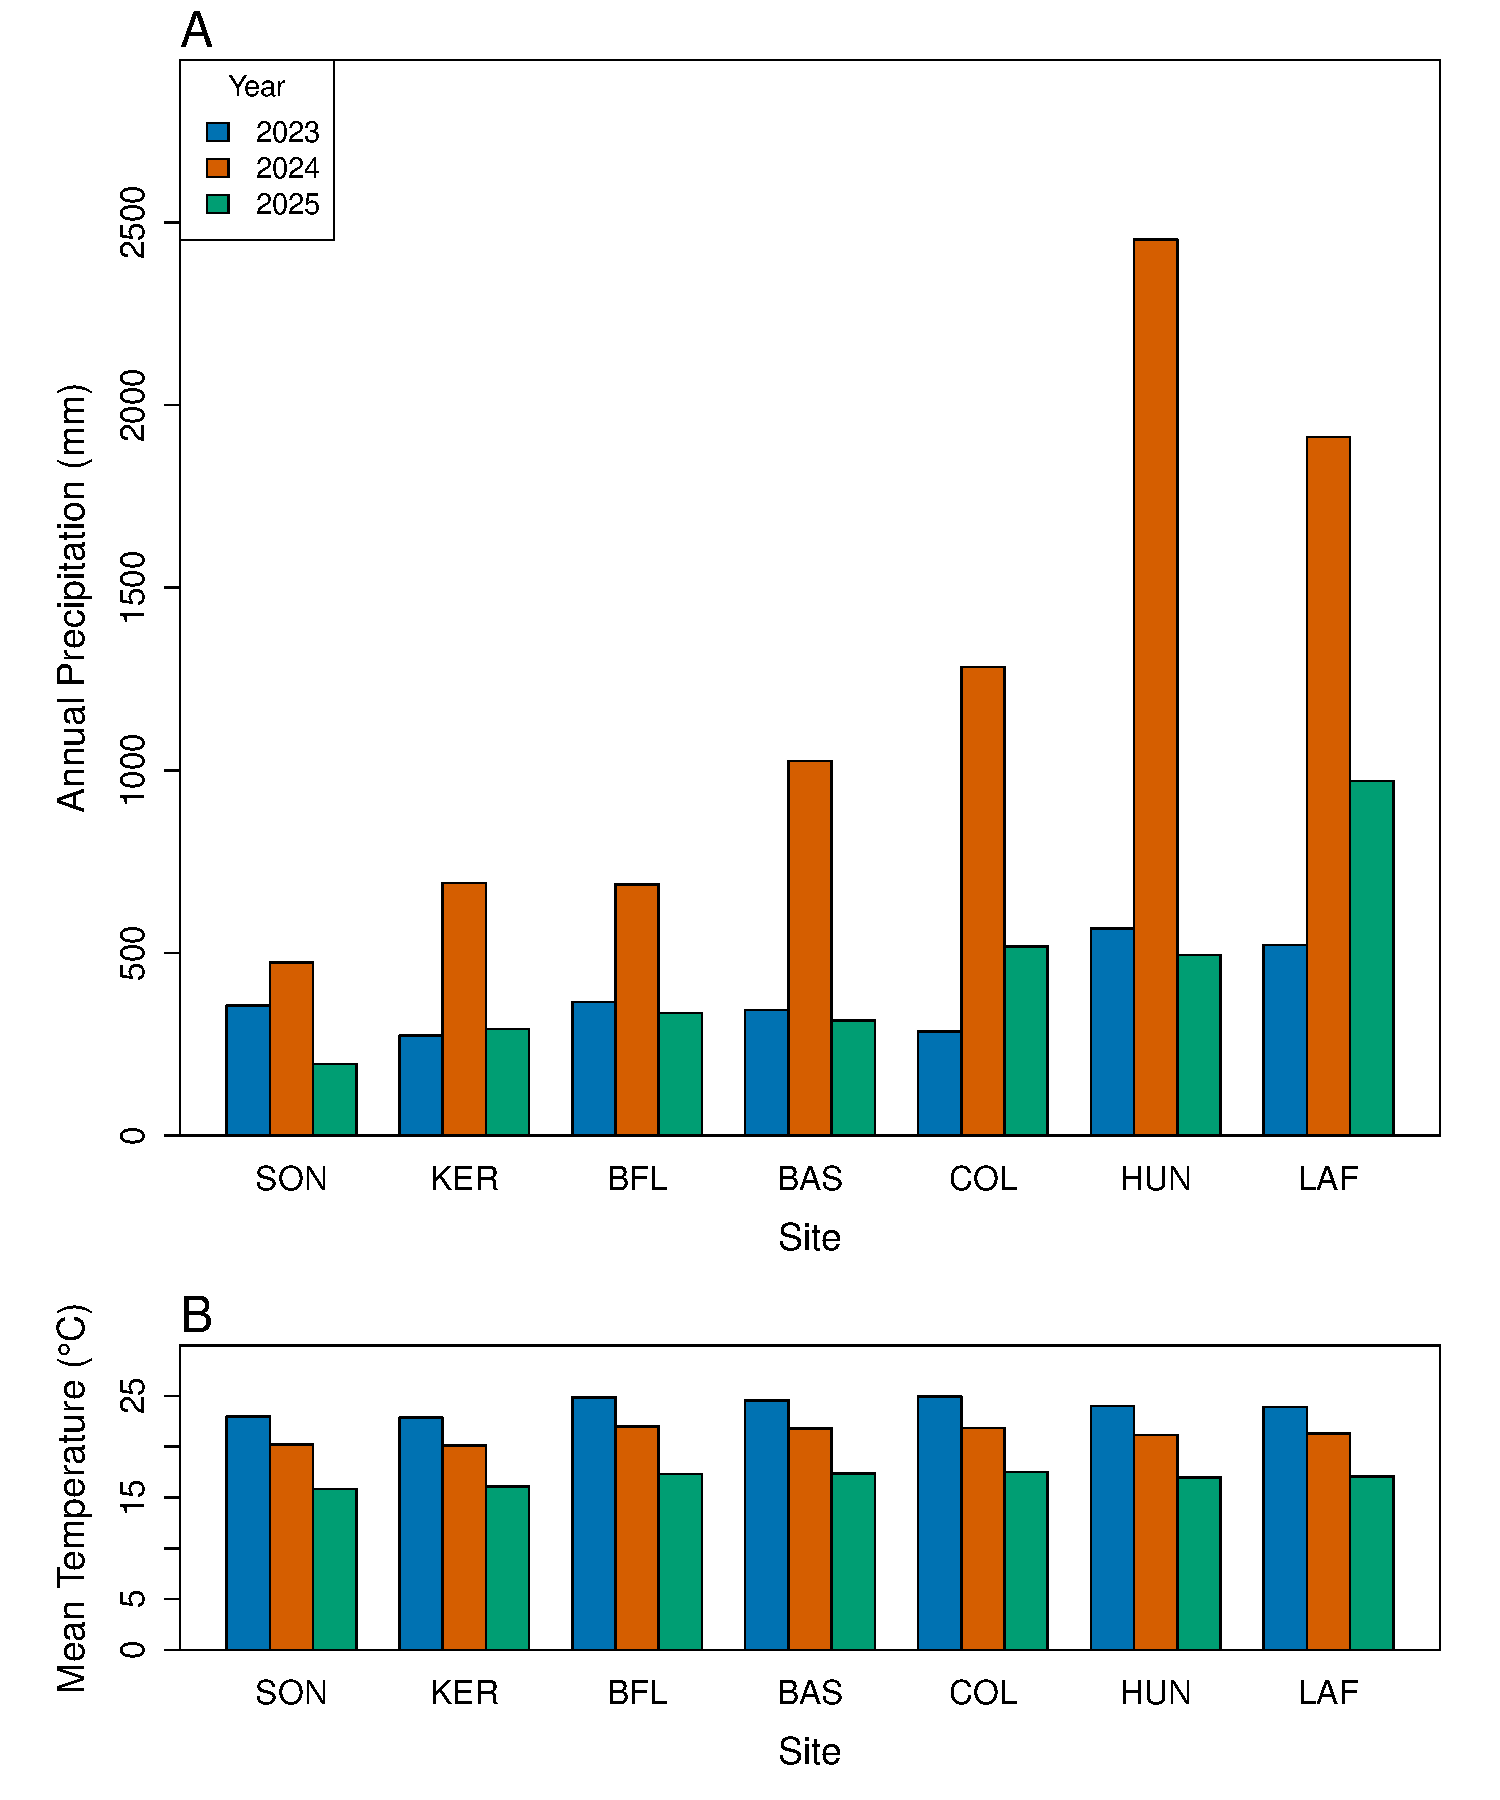
\includegraphics[width=0.8\linewidth]{../Figure/temp_pppt_site_year.pdf}
		\caption[spatial and temporal variation in precipitation and temperature across the experimental sites.] {
		(A) Annual precipitation (mm) and (B) mean temperature (°C) for 2023–2025.
		Sites are arranged from west to east based on longitude.}
		\label{Sup:temp}
\end{figure}
\clearpage  % forces the next figure to start on a new page

\begin{figure}[ht]
\centering
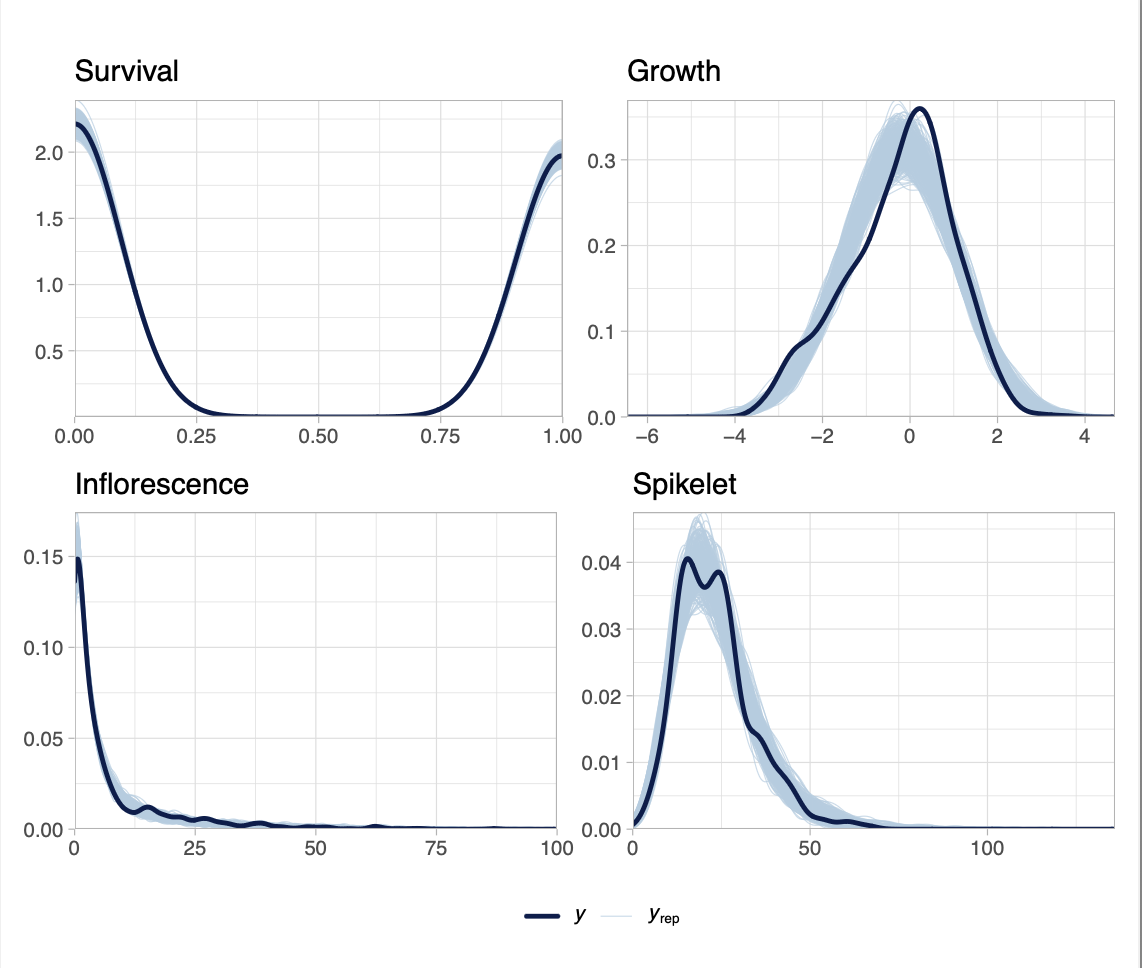
\includegraphics[width=1\textwidth]{../Figure/PPC_linear.png}
\caption[Posterior predictive checks for each vital rate]{
Posterior predictive checks for each vital rate. 
Dark blue lines show observed data ($y$), and light blue lines show replicated datasets generated from posterior predictions ($y_{\text{rep}}$). 
The strong overlap across survival, growth, flowering, and spikelet production indicates adequate model fit for all vital rates.
}
\label{sup:ppc_vital}
\end{figure}

\begin{figure}[H]
		\centering
		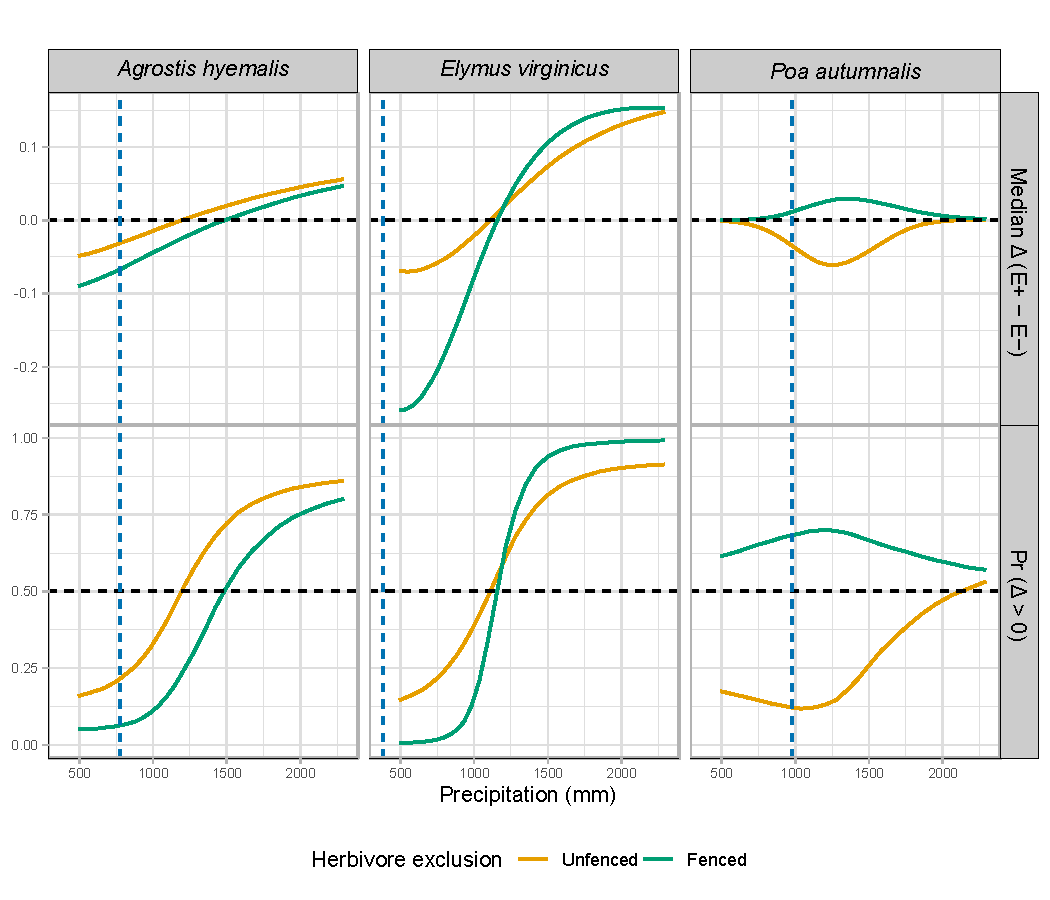
\includegraphics[width=1\linewidth]{../Figure/PrSurvival_diff_stat.pdf}
		\caption[Endophyte effects ($\Delta$) on survival across precipitation gradients with and without herbivory exclusion]
{Predicted effects of endophyte presence (E$^+$) versus absence (E$^-$) on survival across precipitation gradients for three cool-season grasses. 
		Solid lines show the median $\Delta$ (E$^+$ $-$ E$^-$),or the posterior probability that $\Delta > 0$ under fenced and unfenced conditions. 
		Horizontal dashed lines indicate no effect ($\Delta = 0$) or a 50\% probability of benefit. 
		Vertical dashed lines represent the precipitation values at the most westerly natural occurrence of each species, based on GBIF records.}
		\label{sup:survival_delta}
\end{figure}

\begin{figure}[H]
		\centering
		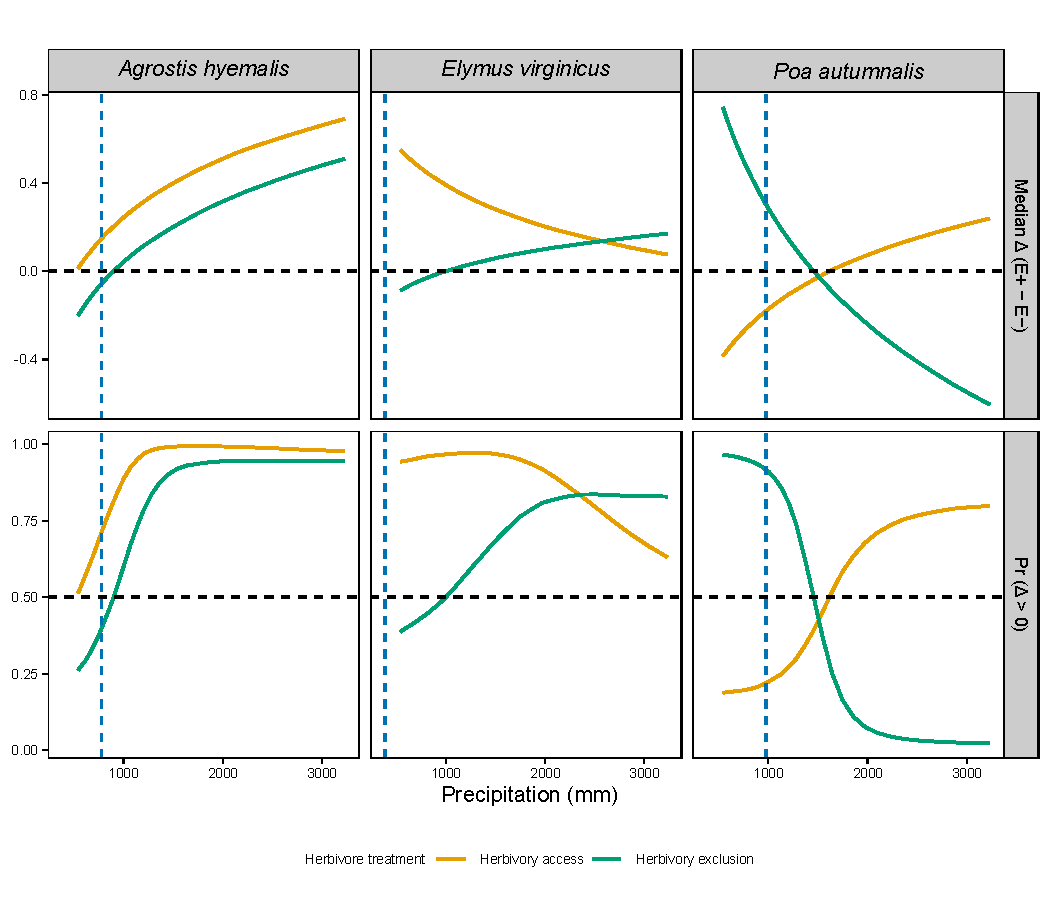
\includegraphics[width=1\linewidth]{../Figure/Growth_diff_stat.pdf}
		\caption[Endophyte effects ($\Delta$) on growth across precipitation gradients with and without herbivory exclusion]{Effects of precipitation and endophyte presence on growth across three cool-season grass species. 
		Lines show the predicted difference in growth between endophyte-present (E$^+$) and endophyte-absent (E$^-$) plants (Median $\Delta$, top row) and the posterior probability that this difference is positive (Pr($\Delta > 0$), bottom row) under fenced and unfenced treatments. Predictions were calculated at the 10th, 25th, 50th, 75th, and 90th percentiles of precipitation observed in the study. Horizontal dashed lines indicate $\Delta = 0$ (top row) and Pr($\Delta > 0$) = 0.5 (bottom row).
		Vertical dashed lines represent the precipitation values at the most westerly natural occurrence of each species, based on GBIF records.}
		\label{sup:growth_delta}
\end{figure}

\begin{figure}[H]
		\centering
		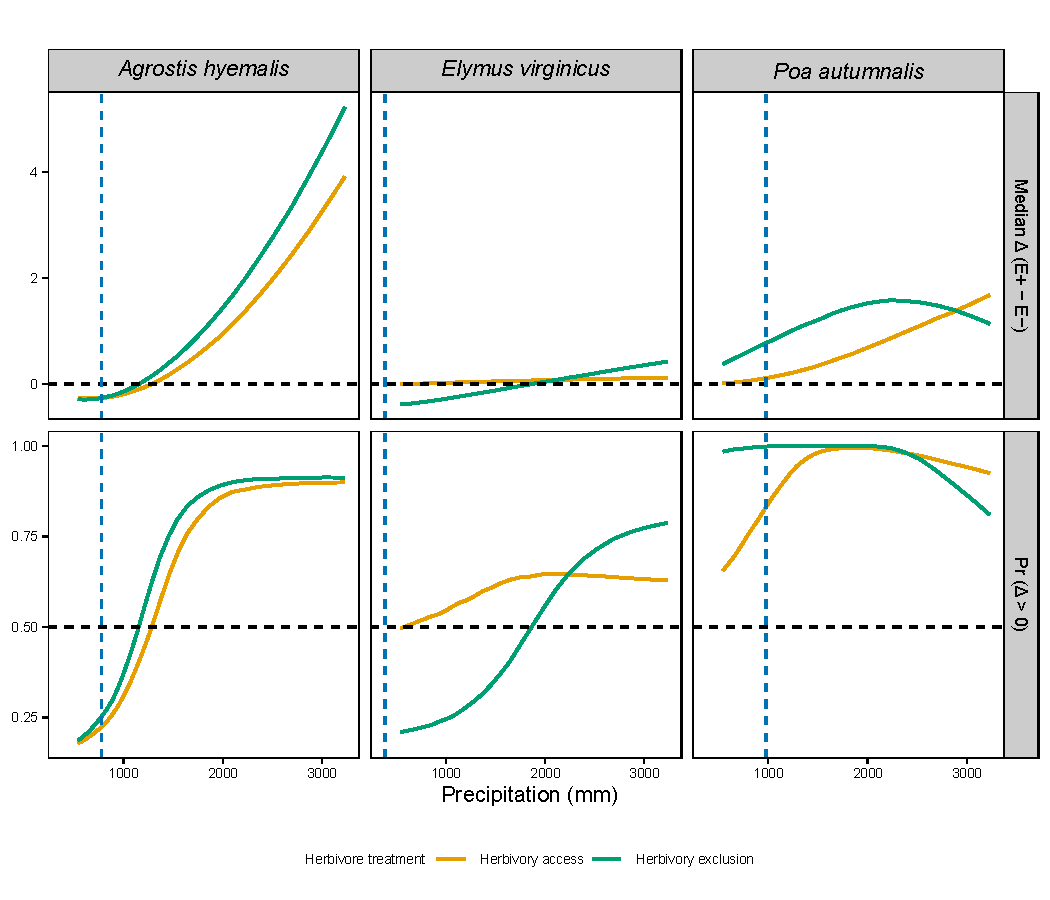
\includegraphics[width=1\linewidth]{../Figure/Inflorescence_diff_stat.pdf}
		\caption[Endophyte effects ($\Delta$) on inflorescence number across precipitation gradients with and without herbivory exclusion.
]{Effects of endophyte infection on flowering output across a precipitation gradient for three cool-season grass species. Lines show the median posterior difference $\Delta$ (E$^{+}$ $-$ E$^{-}$) and the posterior probability that $\Delta > 0$ under fenced (herbivores excluded) and unfenced (herbivores present) conditions. Horizontal dashed lines indicate $\Delta = 0$ for median differences and $\mathrm{Pr}(\Delta > 0) = 0.5$. Endophyte effects were generally positive for \textit{Agrostis hyemalis} and \textit{Poa autumnalis}, but for \textit{Elymus virginicus} benefits were context-dependent, with costs at lower precipitation}
		\label{sup:flowering_delta}
\end{figure}

\begin{figure}[H]
\centering
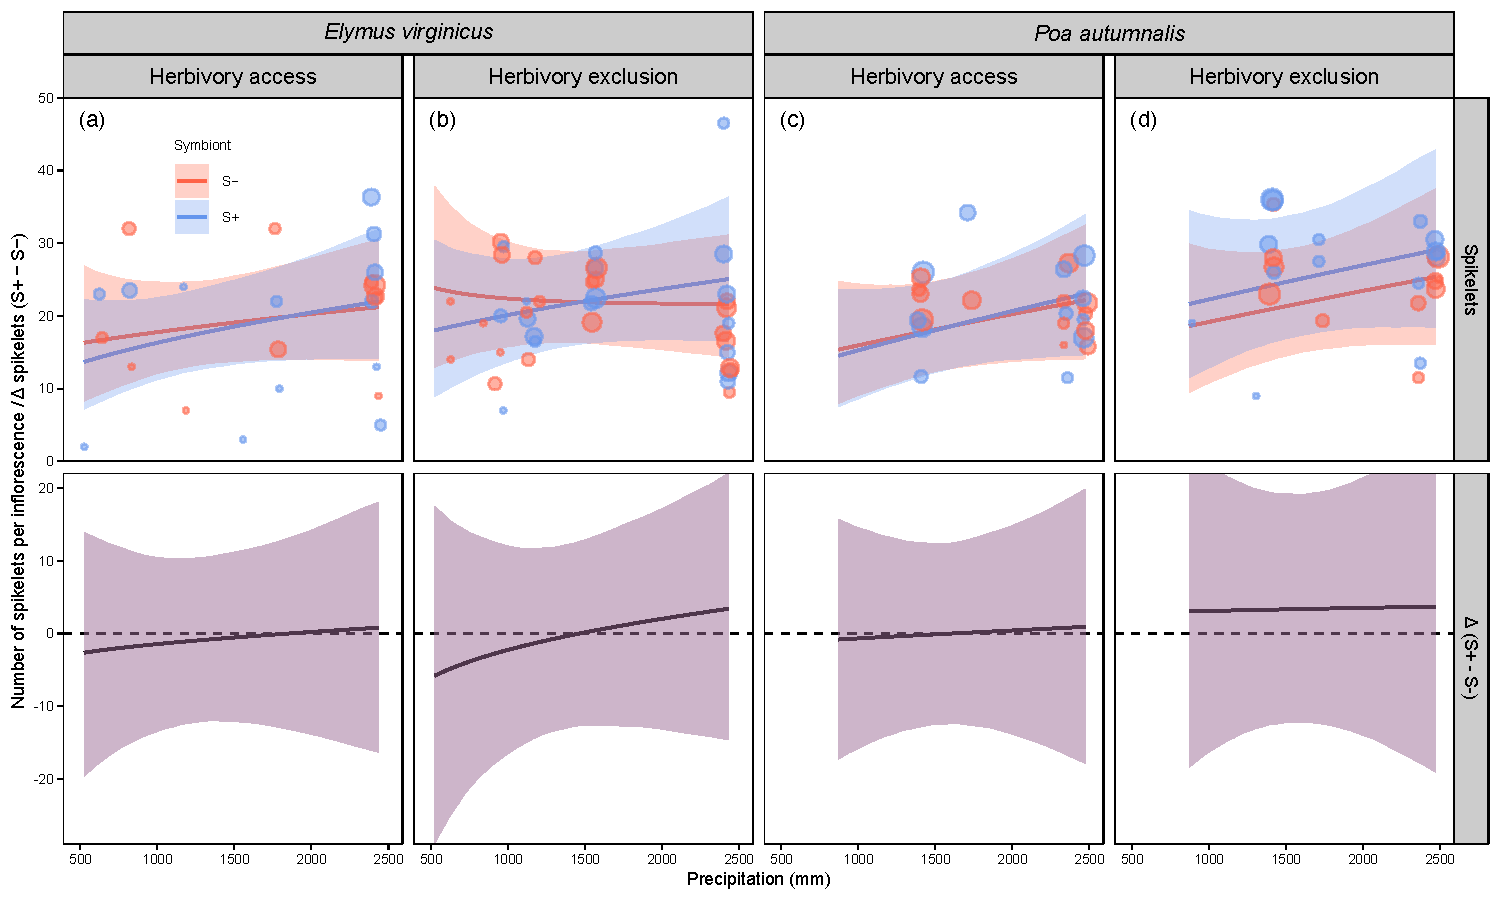
\includegraphics[width=1\textwidth]{../Figure/Spikelet_diff.pdf}
\caption[Endophyte effects ($\Delta$) on spikelet production across precipitation gradients with and without herbivory exclusion]{Predicted number of spikelets (upper panels) and endophyte effect (\(\Delta = \mathrm{E^+ - E^-}\), bottom panels) across precipitation gradients. 
Lines show posterior means for E\(^+\) (blue) and E\(^-\) (red), with shading indicating 90\% credible intervals. 
Points represent mean observed spikelets per plot, slightly jittered for visualization. 
Spikelets were measured for only two species (see Methods for details).  
The dashed line at \(\Delta = 0\) indicates no endophyte effect. 
Panels are organized by species and herbivory treatment (Fenced, Unfenced).}
\label{sup:spikelet}
\end{figure}

\begin{figure}[H]
		\centering
		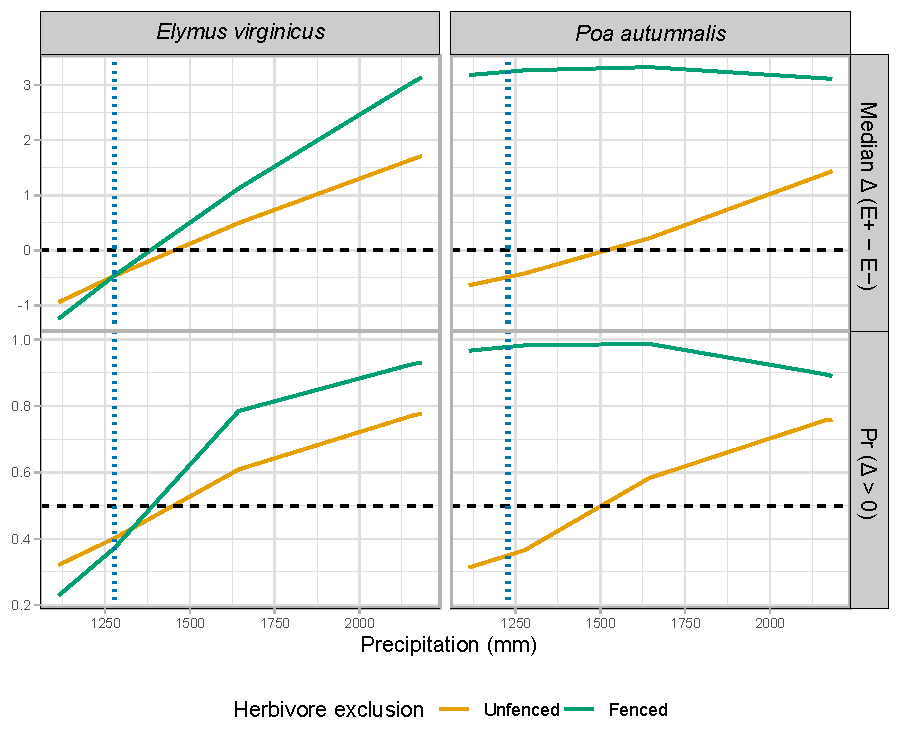
\includegraphics[width=1\linewidth]{../Figure/Spike_diff_stat.pdf}
		\caption[Effects of precipitation and endophyte presence on spikelet with and without herbivory exclusion]{Effects of precipitation and endophyte presence on spikelet (reproductive output) for three cool-season grass species. Median $\Delta$ (E$^{+} - $E$^{-}$) and posterior probability $\mathrm{Pr}(\Delta > 0)$ are shown across precipitation quantiles. Herbivore exclusion treatments are indicated by color (Fenced = herbivores excluded, Unfenced = herbivores had access). Horizontal dashed lines indicate $\Delta = 0$ for medians and $\mathrm{Pr}(\Delta > 0) = 0.5$ for probabilities. Facets separate metrics and species.}
		\label{sup:spike_delta}
\end{figure}

%\begin{figure}[H]
%		\centering
%		
\includegraphics[width=0.50\linewidth]{ppt_surv_coeff.pdf}
%		\caption{Coefficient estimates from Bayesian models linking survival and geographic distance.
%		 Points represent posterior means and lines indicate 95\% credible intervals.
%		 Species abbreviations: \textit{Agrostis hyemalis} (AGHY), \textit{Elymus virginicus} (ELVI), and \textit{Poa autumnalis} (PAOU).
%		 Horizontal dashed lines denote zero effect.}
%		\label{Sup:temp_variation}
%\end{figure}
%
%\begin{figure}[H]
%		\centering
%		
\includegraphics[width=0.50\linewidth]{ppt_grow_coeff.pdf}
%		\caption{Coefficient estimates from Bayesian models linking growth and geographic distance.
%		 Points represent posterior means and lines indicate 95\% credible intervals.
%		 Species abbreviations: \textit{Agrostis hyemalis} (AGHY), \textit{Elymus virginicus} (ELVI), and \textit{Poa autumnalis} (PAOU).
%		 Horizontal dashed lines denote zero effect.}
%		\label{Sup:temp_variation}
%\end{figure}
%
%\begin{figure}[H]
%		\centering
%		
\includegraphics[width=0.50\linewidth]{ppt_flow_coeff.pdf}
%		\caption{Coefficient estimates from Bayesian models linking flowering and geographic distance.
%		 Points represent posterior means and lines indicate 95\% credible intervals.
%		 Species abbreviations: \textit{Agrostis hyemalis} (AGHY), \textit{Elymus virginicus} (ELVI), and \textit{Poa autumnalis} (PAOU).
%		 Horizontal dashed lines denote zero effect.}
%		\label{Sup:temp_variation}
%\end{figure}
%
%\begin{figure}[H]
%		\centering
%		
\includegraphics[width=0.50\linewidth]{ppt_spik_coeff.pdf}
%		\caption{Coefficient estimates from Bayesian models linking flowering and geographic distance.
%		 Points represent posterior means and lines indicate 95\% credible intervals.
%		 Species abbreviations: \textit{Agrostis hyemalis} (AGHY), \textit{Elymus virginicus} (ELVI), and \textit{Poa autumnalis} (PAOU).
%		 Horizontal dashed lines denote zero effect.}
%		\label{Sup:temp_variation}
%\end{figure}
%
%

%\begin{figure}[H]
%		\centering
%		\includegraphics[width=0.95\linewidth]{Figures/fig_pr_past_present_future.pdf}
%		\caption{Precipitation variation across the study sites from 1990 to 2100.
%		ds: Dormant season, dg: Growing season.}
%		\label{Sup:pr_variation}
%\end{figure}
%
%\begin{figure}[H]
%		\centering
%		\includegraphics[width=0.95\linewidth]{Figures/MIROC.pdf}
%		\caption{Past, Observed, present and future (MIROC Model) climate data across the study area.}
%		\label{Sup:projectionMIROC}
%\end{figure}
%
%\begin{figure}[H]
%		\centering
%		\includegraphics[width=0.99\linewidth]{Figures/ACCESS.pdf}
%		\caption{Past, Observed, present and future (ACCESS Model) climate data across the study area.}
%		\label{Sup:projectionACCESS}
%\end{figure}
%
%\begin{figure}[H]
%		\centering
%		\includegraphics[width=0.99\linewidth]{Figures/CESM1.pdf}
%		\caption{Past, Observed, present and future (CESM1 Model) climate data across the study area.}
%		\label{Sup:projectionCESM1}
%\end{figure}
%
%\begin{figure}[H]
%		\centering
%		\includegraphics[width=0.99\linewidth]{Figures/CMCC.pdf}
%		\caption{Past, Observed, present and future (CMCC Model) climate data across the study area.}
%		\label{Sup:projectionCMCC}
%\end{figure}
%
%\begin{figure}[H]
%		\centering
%		\includegraphics[width=0.959\linewidth]{Figures/site_year_weather.pdf}
%		\caption{Climate variation across the study sites during the monitoring period.}
%		\label{Sup:climate_variation}
%\end{figure}


\end{document}
